%%%%%%%%%%%%%%%%%%%%%%%%%%%%%%%%%%%%%%%%%%%%%%%%%%%%%%%%%%%%%%%%%%%%%%%%%%%%%%%%
% Présentation : Des LLM aux agents locaux
% Thème : Formation Club (Beamer avec Miniframes & CambridgeUS)
% Plan détaillé : voir plan.md (timing, démos, sources, checklist J-1)
% Licence : CC BY-NC-SA 4.0 — figures 3Blue1Brown (CC BY-NC-SA, img/README.md)
%%%%%%%%%%%%%%%%%%%%%%%%%%%%%%%%%%%%%%%%%%%%%%%%%%%%%%%%%%%%%%%%%%%%%%%%%%%%%%%%

\documentclass[
	11pt,
	aspectratio=169
]{beamer}

%----------------------------------------------------------------------------------------
%	PACKAGES ET CONFIGURATION LINGUISTIQUE
%----------------------------------------------------------------------------------------
\usepackage[utf8]{inputenc}
\usepackage[T1]{fontenc}
\usepackage[french]{babel}
\usepackage{booktabs}
\usepackage{tikz}
\usetikzlibrary{arrows.meta, positioning, shapes.geometric, backgrounds, fit}
\usepackage{listings}
\usepackage{ccicons} % Icônes Creative Commons
\usepackage{ulem}

%----------------------------------------------------------------------------------------
%	SÉLECTION DU THÈME ET POLICES
%----------------------------------------------------------------------------------------
\usetheme{CambridgeUS}
\useinnertheme{circles}
\useoutertheme{miniframes} % Active les points de navigation en haut

\usepackage[default]{opensans}

% Palette « LLM » personnalisée
\definecolor{llmblue}{RGB}{77, 107, 254}    % Bleu DeepSeek
\definecolor{llmdark}{RGB}{30, 34, 45}      % Gris ardoise
\definecolor{llmlight}{RGB}{246, 248, 250}  % Gris clair de fond
\definecolor{llmgreen}{RGB}{40, 167, 69}    % Vert succès
\definecolor{llmorange}{RGB}{227, 137, 52}  % Orange avertissement
\definecolor{llmborder}{RGB}{209, 213, 218} % Bordure neutre

% Pied de page infolines avec les miniframes en haut (comme le support Git)
\makeatletter
\setbeamertemplate{footline}{
  \leavevmode%
  \hbox{%
  \begin{beamercolorbox}[wd=.333333\paperwidth,ht=2.25ex,dp=1ex,center]{author in head/foot}%
    \usebeamerfont{author in head/foot}\insertshortauthor
  \end{beamercolorbox}%
  \begin{beamercolorbox}[wd=.333333\paperwidth,ht=2.25ex,dp=1ex,center]{title in head/foot}%
    \usebeamerfont{title in head/foot}\insertshorttitle
  \end{beamercolorbox}%
  \begin{beamercolorbox}[wd=.333333\paperwidth,ht=2.25ex,dp=1ex,right]{date in head/foot}%
    \usebeamerfont{date in head/foot}\insertshortdate{}\hspace*{1.5em}
    \insertframenumber{} / \inserttotalframenumber\hspace*{1.5ex}
  \end{beamercolorbox}}%
  \vskip0pt%
}
\makeatother

%----------------------------------------------------------------------------------------
%	CONFIGURATION LISTINGS (CORRECTION DES ACCENTS UTF-8)
%----------------------------------------------------------------------------------------
\lstdefinestyle{llmstyle}{
    basicstyle=\ttfamily\footnotesize,
    backgroundcolor=\color{llmlight},
    frame=single,
    rulecolor=\color{llmborder},
    keywordstyle=\color{llmblue}\bfseries,
    commentstyle=\color{gray}\itshape,
    stringstyle=\color{llmgreen},
    breaklines=true,
    showstringspaces=false,
    inputencoding=utf8,
    extendedchars=true,
    literate=
        {á}{{\'a}}1 {é}{{\'e}}1 {í}{{\'i}}1 {ó}{{\'o}}1 {ú}{{\'u}}1
        {Á}{{\'A}}1 {É}{{\'E}}1 {Í}{{\'I}}1 {Ó}{{\'O}}1 {Ú}{{\'U}}1
        {à}{{\`a}}1 {è}{{\`e}}1 {ì}{{\`i}}1 {ò}{{\`o}}1 {ù}{{\`u}}1
        {À}{{\`A}}1 {È}{{\`E}}1 {Ì}{{\`I}}1 {Ò}{{\`O}}1 {Ù}{{\`U}}1
        {ä}{{\"a}}1 {ë}{{\"e}}1 {ï}{{\"i}}1 {ö}{{\"o}}1 {ü}{{\"u}}1
        {Ä}{{\"A}}1 {Ë}{{\"E}}1 {Ï}{{\"I}}1 {Ö}{{\"O}}1 {Ü}{{\"U}}1
        {â}{{\^a}}1 {ê}{{\^e}}1 {î}{{\^i}}1 {ô}{{\^o}}1 {û}{{\^u}}1
        {Â}{{\^A}}1 {Ê}{{\^E}}1 {Î}{{\^I}}1 {Ô}{{\^O}}1 {Û}{{\^U}}1
        {œ}{{\oe}}1 {Œ}{{\OE}}1 {æ}{{\ae}}1 {Æ}{{\AE}}1
        {ç}{{\c{c}}}1 {Ç}{{\c{C}}}1
        {«}{{\og}}1 {»}{{\fg}}1
}
\lstset{style=llmstyle}

% Style commun pour les schémas TikZ « pile logicielle »
\tikzset{
  box/.style={draw=llmborder, fill=llmlight, rounded corners, align=center, font=\small, inner sep=6pt},
  hbox/.style={box, fill=llmblue!10, draw=llmblue},
  arr/.style={-{Stealth[length=2mm]}, thick, llmdark}
}

%----------------------------------------------------------------------------------------
%	MÉTADONNÉES DE LA PRÉSENTATION
%----------------------------------------------------------------------------------------
\title[Des LLM aux agents locaux]{Des LLM aux agents locaux}
\subtitle{Formation Robotech --- du fonctionnement interne au modèle local, puis à son harnais}
\author[Ahmed pour Robotech]{Ahmed}
\institute[Robotech]{\url{https://github.com/Robotech-Lillois}}
\date[\today \quad \ccbyncsa]{\today}

% Logo sur la première page
\titlegraphic{
    \vspace{-0.5cm}
    \IfFileExists{./img/logo.png}{%
        
\includegraphics[height=1.4cm,keepaspectratio]{./img/logo.png}%
    }{%
        \fbox{\color{llmdark}\small\strut Emplacement ./img/logo.png}%
    }
}

\setbeamertemplate{headline}{%
    \leavevmode%
    \begin{beamercolorbox}[wd=\paperwidth,ht=2.5ex,dp=3.0ex]{section in head/foot}%
        \insertnavigation{\dimexpr\paperwidth - 1.5cm\relax}%
        \hfill%
        \IfFileExists{./img/logo.png}{%
            \raisebox{-2.5ex}{
\includegraphics[height=4.5ex,keepaspectratio]{./img/logo.png}}%
        }{%
            \fbox{\tiny .\/img\/logo}%
        }%
        \hspace*{0.4cm}%
    \end{beamercolorbox}%
}

%----------------------------------------------------------------------------------------
%	DÉBUT DU DOCUMENT
%----------------------------------------------------------------------------------------
\begin{document}

%========================================================================================
% SLIDE 1 : TITRE
%========================================================================================
\begin{frame}
    \titlepage
    \vspace{-0.6cm}
    \begin{center}
        \footnotesize
        \ccbyncsa\ Ce support est mis à disposition sous licence \textbf{CC BY-NC-SA 4.0} --- figures : 3Blue1Brown
    \end{center}
\end{frame}

%========================================================================================
% SLIDE 2 : SOMMAIRE
%========================================================================================
\begin{frame}
    \frametitle{Sommaire}
    \tableofcontents
\end{frame}

%========================================================================================
\section{Introduction}
%========================================================================================

\begin{frame}
    \frametitle{Ce que vous saurez faire dans 2 heures}
    \begin{enumerate}
        \item \textbf{Expliquer} ce qui se passe dans un LLM quand il « parle » \\
        (tokens $\rightarrow$ plongements $\rightarrow$ attention $\rightarrow$ mot suivant)
        \item \textbf{Faire tourner} un modèle localement avec llama.cpp \\
        (choisir taille, quantification et contexte selon \emph{votre} machine)
        \item \textbf{Comprendre un agent} : la différence entre un chat et une boucle d'agent, et brancher un modèle local sur un harnais (DeepSeek Harness)
    \end{enumerate}
    \vspace{0.3cm}
    \begin{alertblock}{}
        Prérequis : ligne de commande (la formation Git suffit). Aucune maths au-delà du lycée.
    \end{alertblock}
\end{frame}

\begin{frame}
    \frametitle{Pourquoi faire tourner des modèles \emph{en local} ?}
    \begin{columns}[t]
        \begin{column}{0.48\textwidth}
            \begin{block}{\centering \textbf{Local}}
                \begin{itemize}\setlength\itemsep{0.3em}
                    \item Confidentialité : les données ne sortent pas
                    \item Coût marginal nul, pas de limite de débit
                    \item Fonctionne hors ligne (démos, terrain)
                    \item Contrôle et compréhension : excellent pour apprendre
                \end{itemize}
            \end{block}
        \end{column}
        \begin{column}{0.48\textwidth}
            \begin{exampleblock}{\centering \textbf{Cloud / API}}
                \begin{itemize}\setlength\itemsep{0.3em}
                    \item Capacité brute (les très gros modèles)
                    \item Aucune machine à dimensionner
                    \item Raisonnement avancé, multimodal large
                \end{itemize}
            \end{exampleblock}
        \end{column}
    \end{columns}
    \vspace{0.1cm}
    \begin{center}
        Ce n'est pas une religion, c'est un \textbf{compromis} --- et aujourd'hui le local est \emph{réellement} utile.
    \end{center}
\end{frame}

\begin{frame}
    \frametitle{La pile logicielle en une image}
    \begin{columns}[c]
        \begin{column}{0.55\textwidth}
            \centering
            \begin{tikzpicture}
                \node[hbox] (harness) {\textbf{Harnais d'agent}\\ \scriptsize dsh, Claude Code, Codex\dots};
                \node[box, below=0.5cm of harness] (iface) {\textbf{Interface}\\ \scriptsize CLI, API OpenAI-compatible, web UI};
                \node[box, below=0.5cm of iface] (runner) {\textbf{Runner}\\ \scriptsize llama.cpp, Ollama, LM Studio, vLLM};
                \node[box, below=0.5cm of runner] (model) {\textbf{Modèle}\\ \scriptsize poids GGUF (Qwen3.5, Gemma 4\dots)};
                \draw[arr] (model) -- (runner);
                \draw[arr] (runner) -- (iface);
                \draw[arr] (iface) -- (harness);
            \end{tikzpicture}
        \end{column}
        \begin{column}{0.42\textwidth}
            \begin{itemize}\setlength\itemsep{0.6em}
                \item Ollama et LM Studio \emph{sont} llama.cpp sous le capot
                \item Même modèle, même quantification, même GPU $\Rightarrow$ la vitesse ne change pas, seuls les \emph{ wrappers } diffèrent
                \item Le dénominateur commun : l'\textbf{API compatible OpenAI}
            \end{itemize}
        \end{column}
    \end{columns}
\end{frame}

\begin{frame}
    \frametitle{Le fil rouge de la session}
    \begin{center}
        {\Large \texttt{agent = modèle + harnais}}
    \end{center}
    \bigskip
    \begin{itemize}\setlength\itemsep{0.5em}
        \item Un LLM est un \textbf{prédicteur du token suivant} : sans mémoire, sans outils, il ne produit que du texte
        \item Tout le reste (chat, outils, actions sur plusieurs étapes) est du \textbf{logiciel autour} : c'est le harnais
        \item Programme : \textbf{1.} ce qui se passe dans le modèle --- \textbf{2.} le faire tourner chez soi --- \textbf{3.} l'agent autour
    \end{itemize}
\end{frame}

%========================================================================================
\section{Comprendre un LLM}
%========================================================================================
% Sources figures et concepts : 3Blue1Brown, « Attention in transformers,
% step-by-step » (Deep Learning ch. 6) — https://www.3blue1brown.com/lessons/attention

\begin{frame}
    \frametitle{La prédiction du token suivant}
    \begin{itemize}\setlength\itemsep{0.5em}
        \item Objectif du modèle : étant donné un texte, \textbf{prédire ce qui vient ensuite}
        \item Le texte est d'abord découpé en \textbf{tokens} --- souvent des morceaux de mots, pas des mots entiers
        \item Le modèle établit un \textbf{classement de tous les mots possibles} : ceux qui collent au contexte ont plus de chances de sortir
        \item On tire dans ce classement (plus ou moins au hasard), puis on recommence $\Rightarrow$ une « conversation »
    \end{itemize}
    \vfill
    \begin{center}
        \begin{tikzpicture}
            \node[box] (t1) {\texttt{"Le chat mange le"}};
            \node[box, right=0.5cm of t1] (m) {\textbf{LLM}};
            \node[box, right=0.5cm of m] (t2) {\texttt{"poisson"} (62\%), "gâteau" (9\%)\dots};
            \draw[arr] (t1) -- (m);
            \draw[arr] (m) -- (t2);
        \end{tikzpicture}
    \end{center}
\end{frame}

\begin{frame}
    \frametitle{Les plongements (embeddings)}
    \begin{columns}[c]
        \begin{column}{0.52\textwidth}
            \centering
            \IfFileExists{./img/Embeddings.jpg}{%
                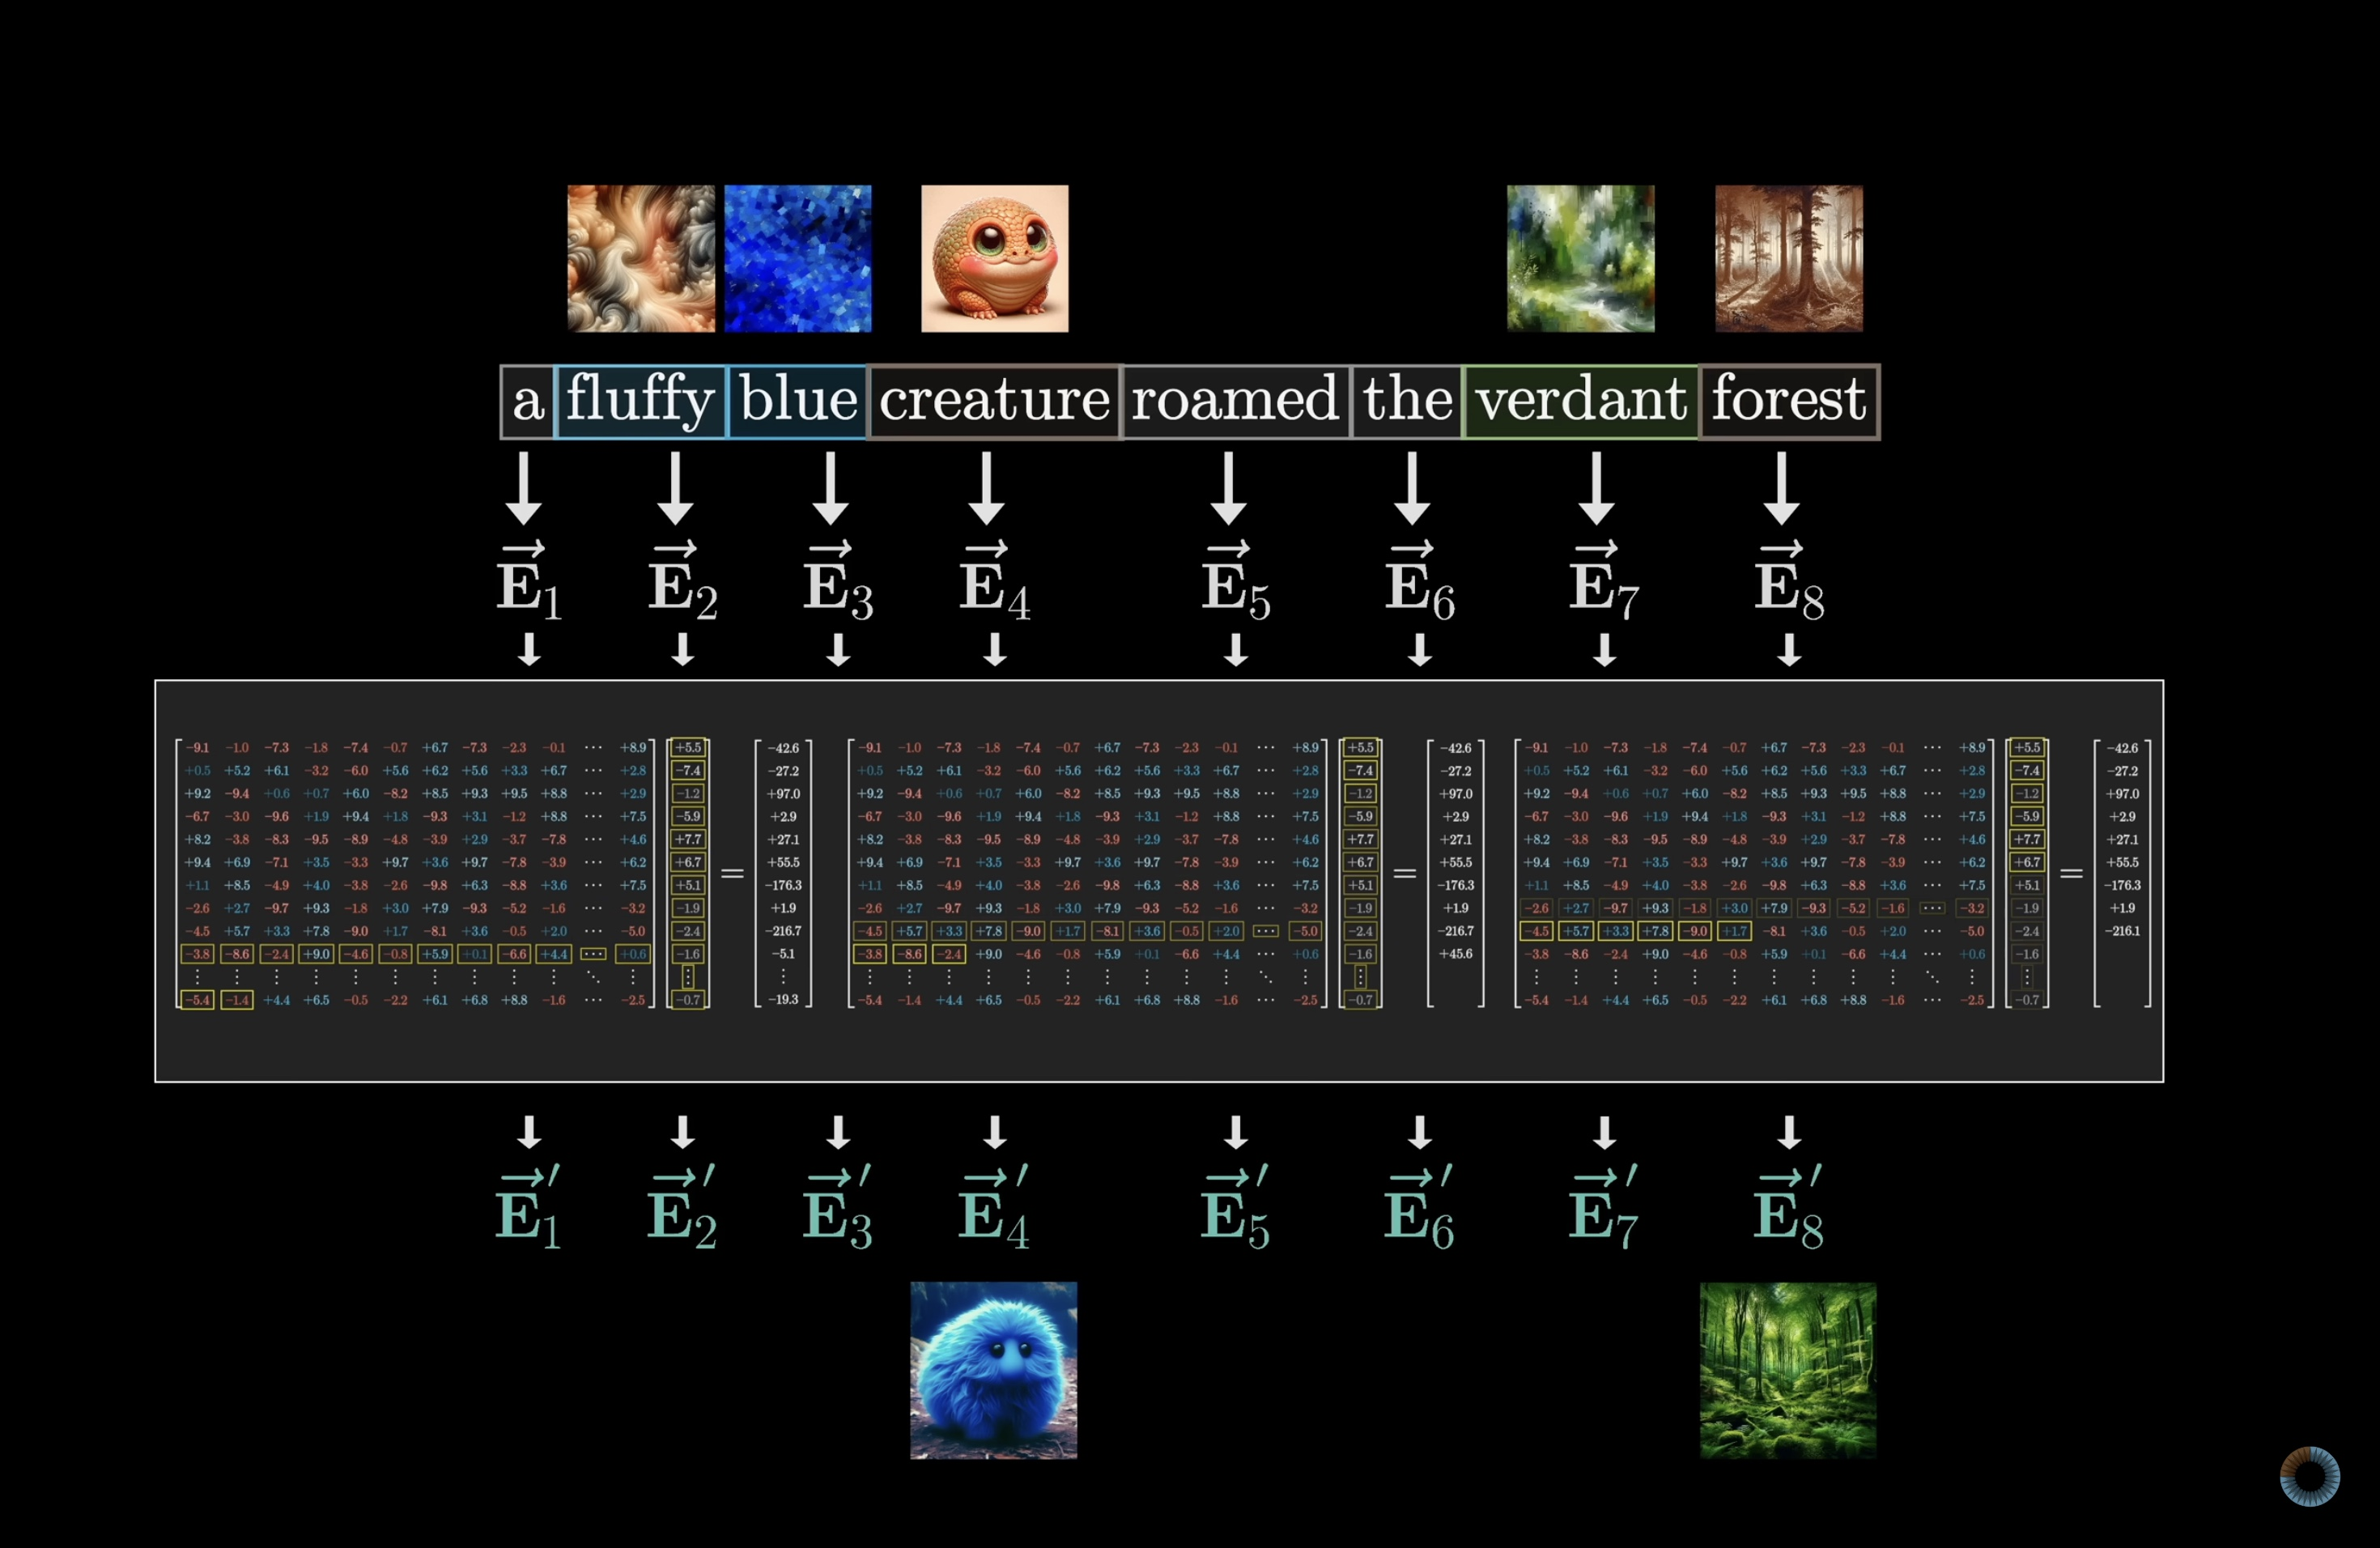
\includegraphics[height=0.72\textheight,width=0.95\linewidth,keepaspectratio]{./img/Embeddings.jpg}%
            }{%
                \fbox{\begin{minipage}[c][3cm][c]{0.9\linewidth}\centering Image \texttt{./img/Embeddings.jpg} manquante\end{minipage}}%
            }
        \end{column}
        \begin{column}{0.44\textwidth}
            \begin{itemize}\setlength\itemsep{0.5em}
                \item Chaque token devient une \textbf{longue liste de nombres} --- un \emph{vecteur} --- : c'est son \textbf{plongement} (embedding)
                \item Certains aspects du sens correspondent à des \textbf{directions} dans cet espace (ex. \emph{king} et \emph{queen} partagent une direction « genre »)
                \item À l'entrée, cette liste ne connaît \emph{que} le token --- pas encore son contexte
            \end{itemize}
        \end{column}
    \end{columns}
\end{frame}

\begin{frame}
    \frametitle{Un mot, plusieurs sens}
    \begin{columns}[c]
        \begin{column}{0.55\textwidth}
            \centering
            \IfFileExists{./img/MoleExample.jpg}{%
                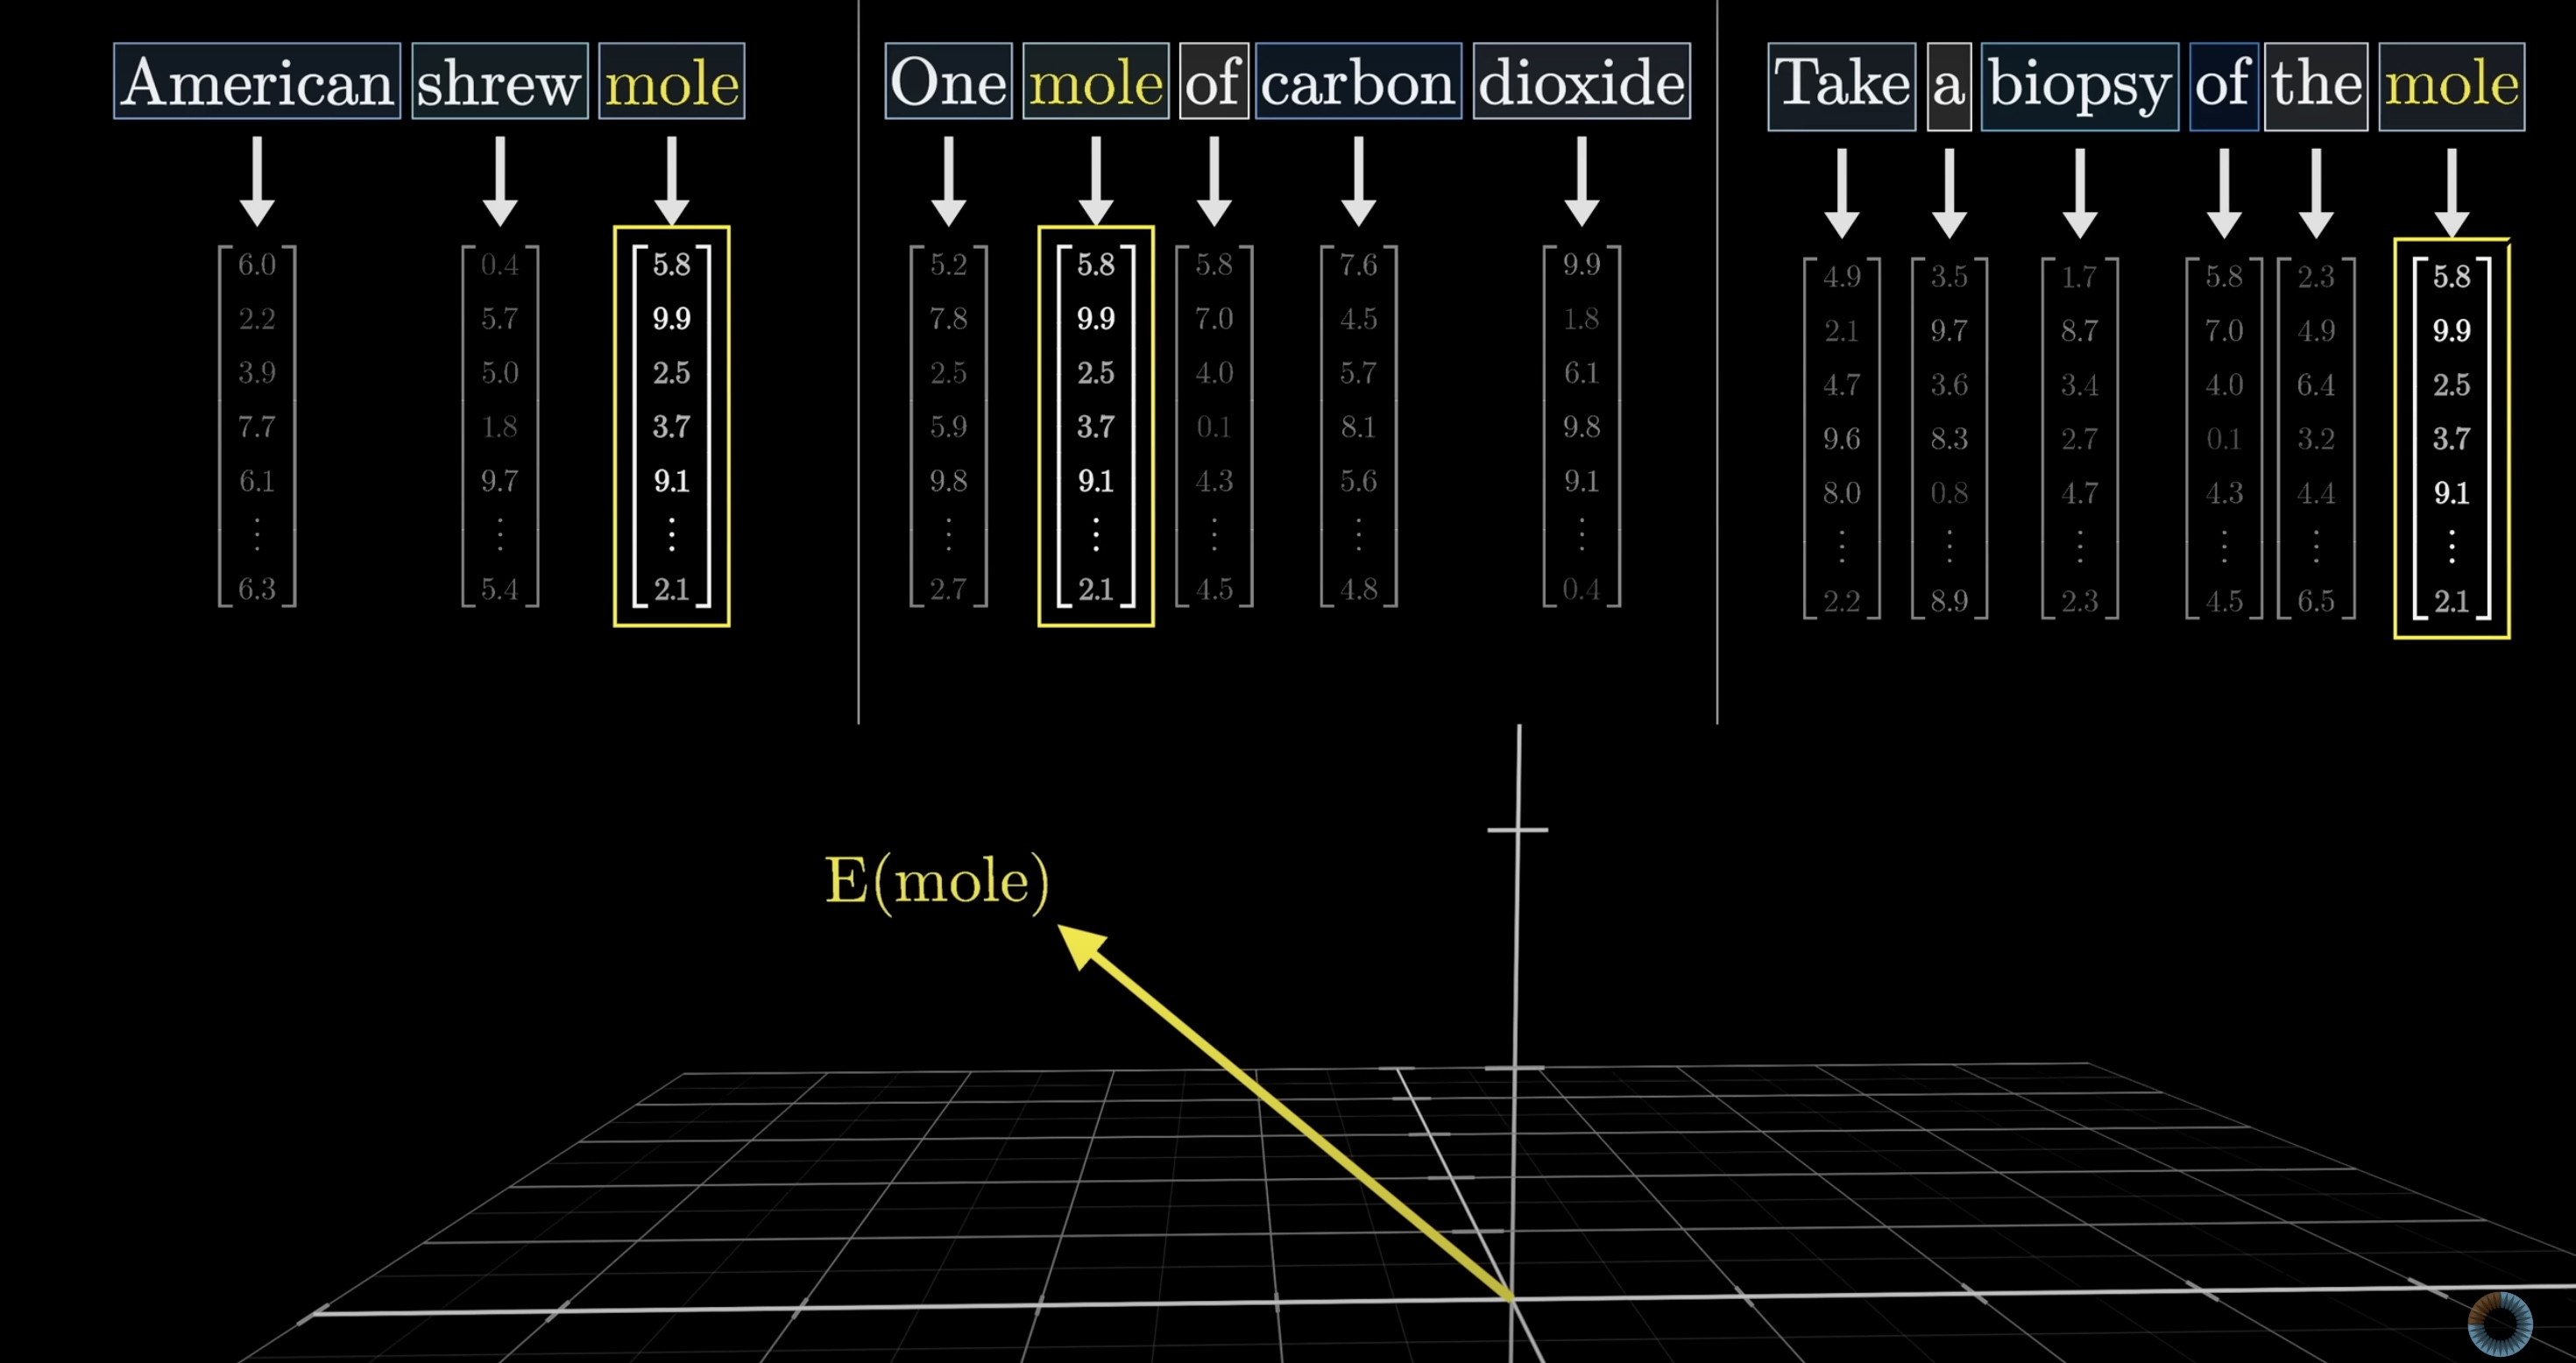
\includegraphics[height=0.75\textheight,width=0.95\linewidth,keepaspectratio]{./img/MoleExample.jpg}%
            }{%
                \fbox{\begin{minipage}[c][3cm][c]{0.9\linewidth}\centering Image \texttt{./img/MoleExample.jpg} manquante\end{minipage}}%
            }
        \end{column}
        \begin{column}{0.42\textwidth}
            \textbf{mole} : \emph{American shrew mole} / \emph{one mole of CO$_2$} / \emph{a biopsy of the mole}\\[0.4em]
            Avant l'attention, le vecteur de « mole » est \emph{identique} dans les trois phrases.\\[0.4em]
            Il faut un mécanisme pour que les voisins \emph{passent de l'information} au vecteur.
        \end{column}
    \end{columns}
\end{frame}

\begin{frame}
    \frametitle{L'information voyage loin}
    \begin{columns}[c]
        \begin{column}{0.55\textwidth}
            \centering
            \IfFileExists{./img/TowerExample.jpg}{%
                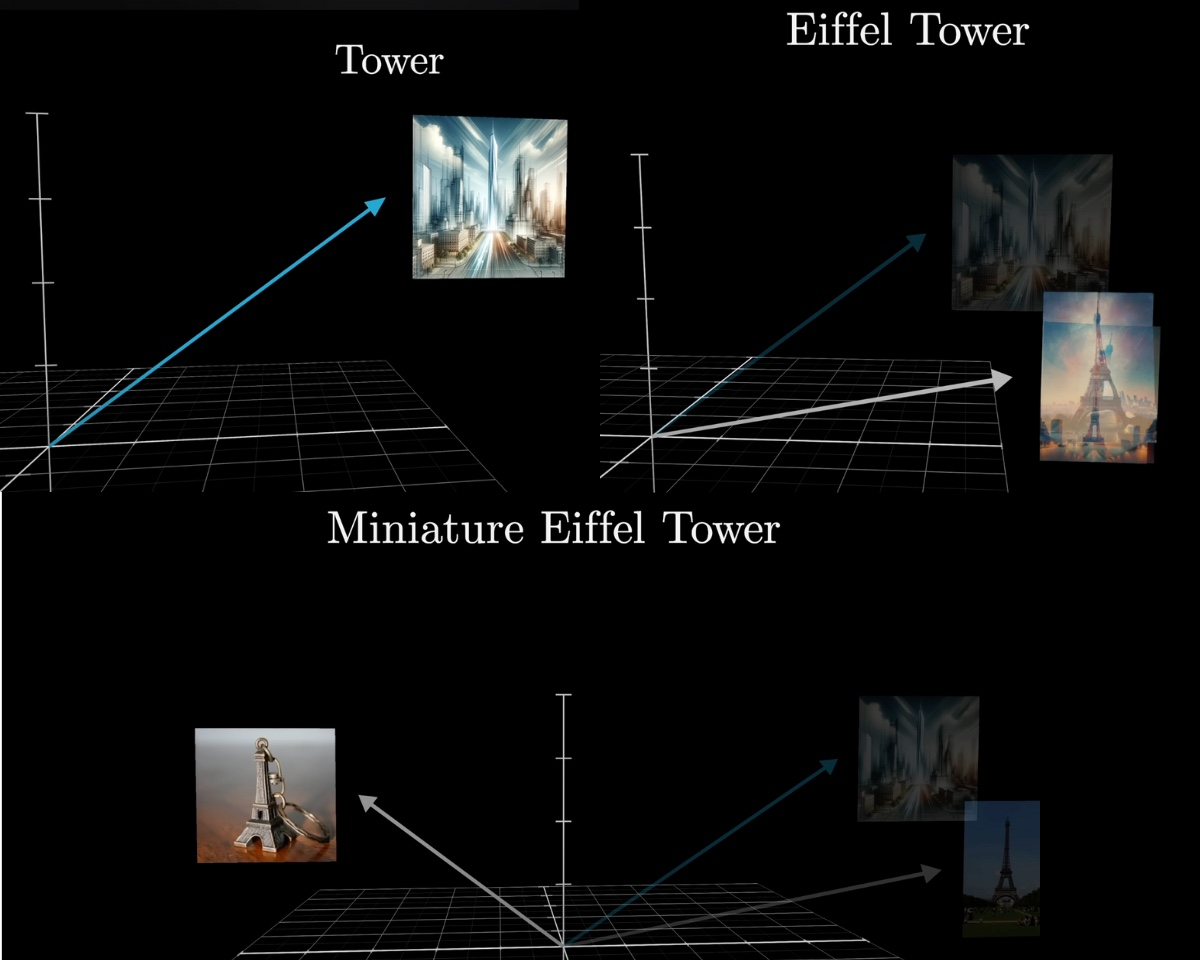
\includegraphics[height=0.62\textheight,width=0.95\linewidth,keepaspectratio]{./img/TowerExample.jpg}%
            }{%
                \fbox{\begin{minipage}[c][3cm][c]{0.9\linewidth}\centering Image \texttt{./img/TowerExample.jpg} manquante\end{minipage}}%
            }
        \end{column}
        \begin{column}{0.42\textwidth}
            \emph{tower} + \emph{Eiffel} $\rightarrow$ Paris, fer \dots puis + \emph{miniature} $\rightarrow$ plus du tout « grand et haut ».\\[0.6em]
            Et pour finir un roman policier par \og therefore the murderer was \dots\fg\ : le dernier vecteur doit avoir absorbé \textbf{tout le contexte pertinent}.
        \end{column}
    \end{columns}
\end{frame}

\begin{frame}
    \frametitle{L'attention : requêtes, clés, valeurs}
    \begin{columns}[c]
        \begin{column}{0.52\textwidth}
            \centering
            \IfFileExists{./img/SingleHead.jpg}{%
                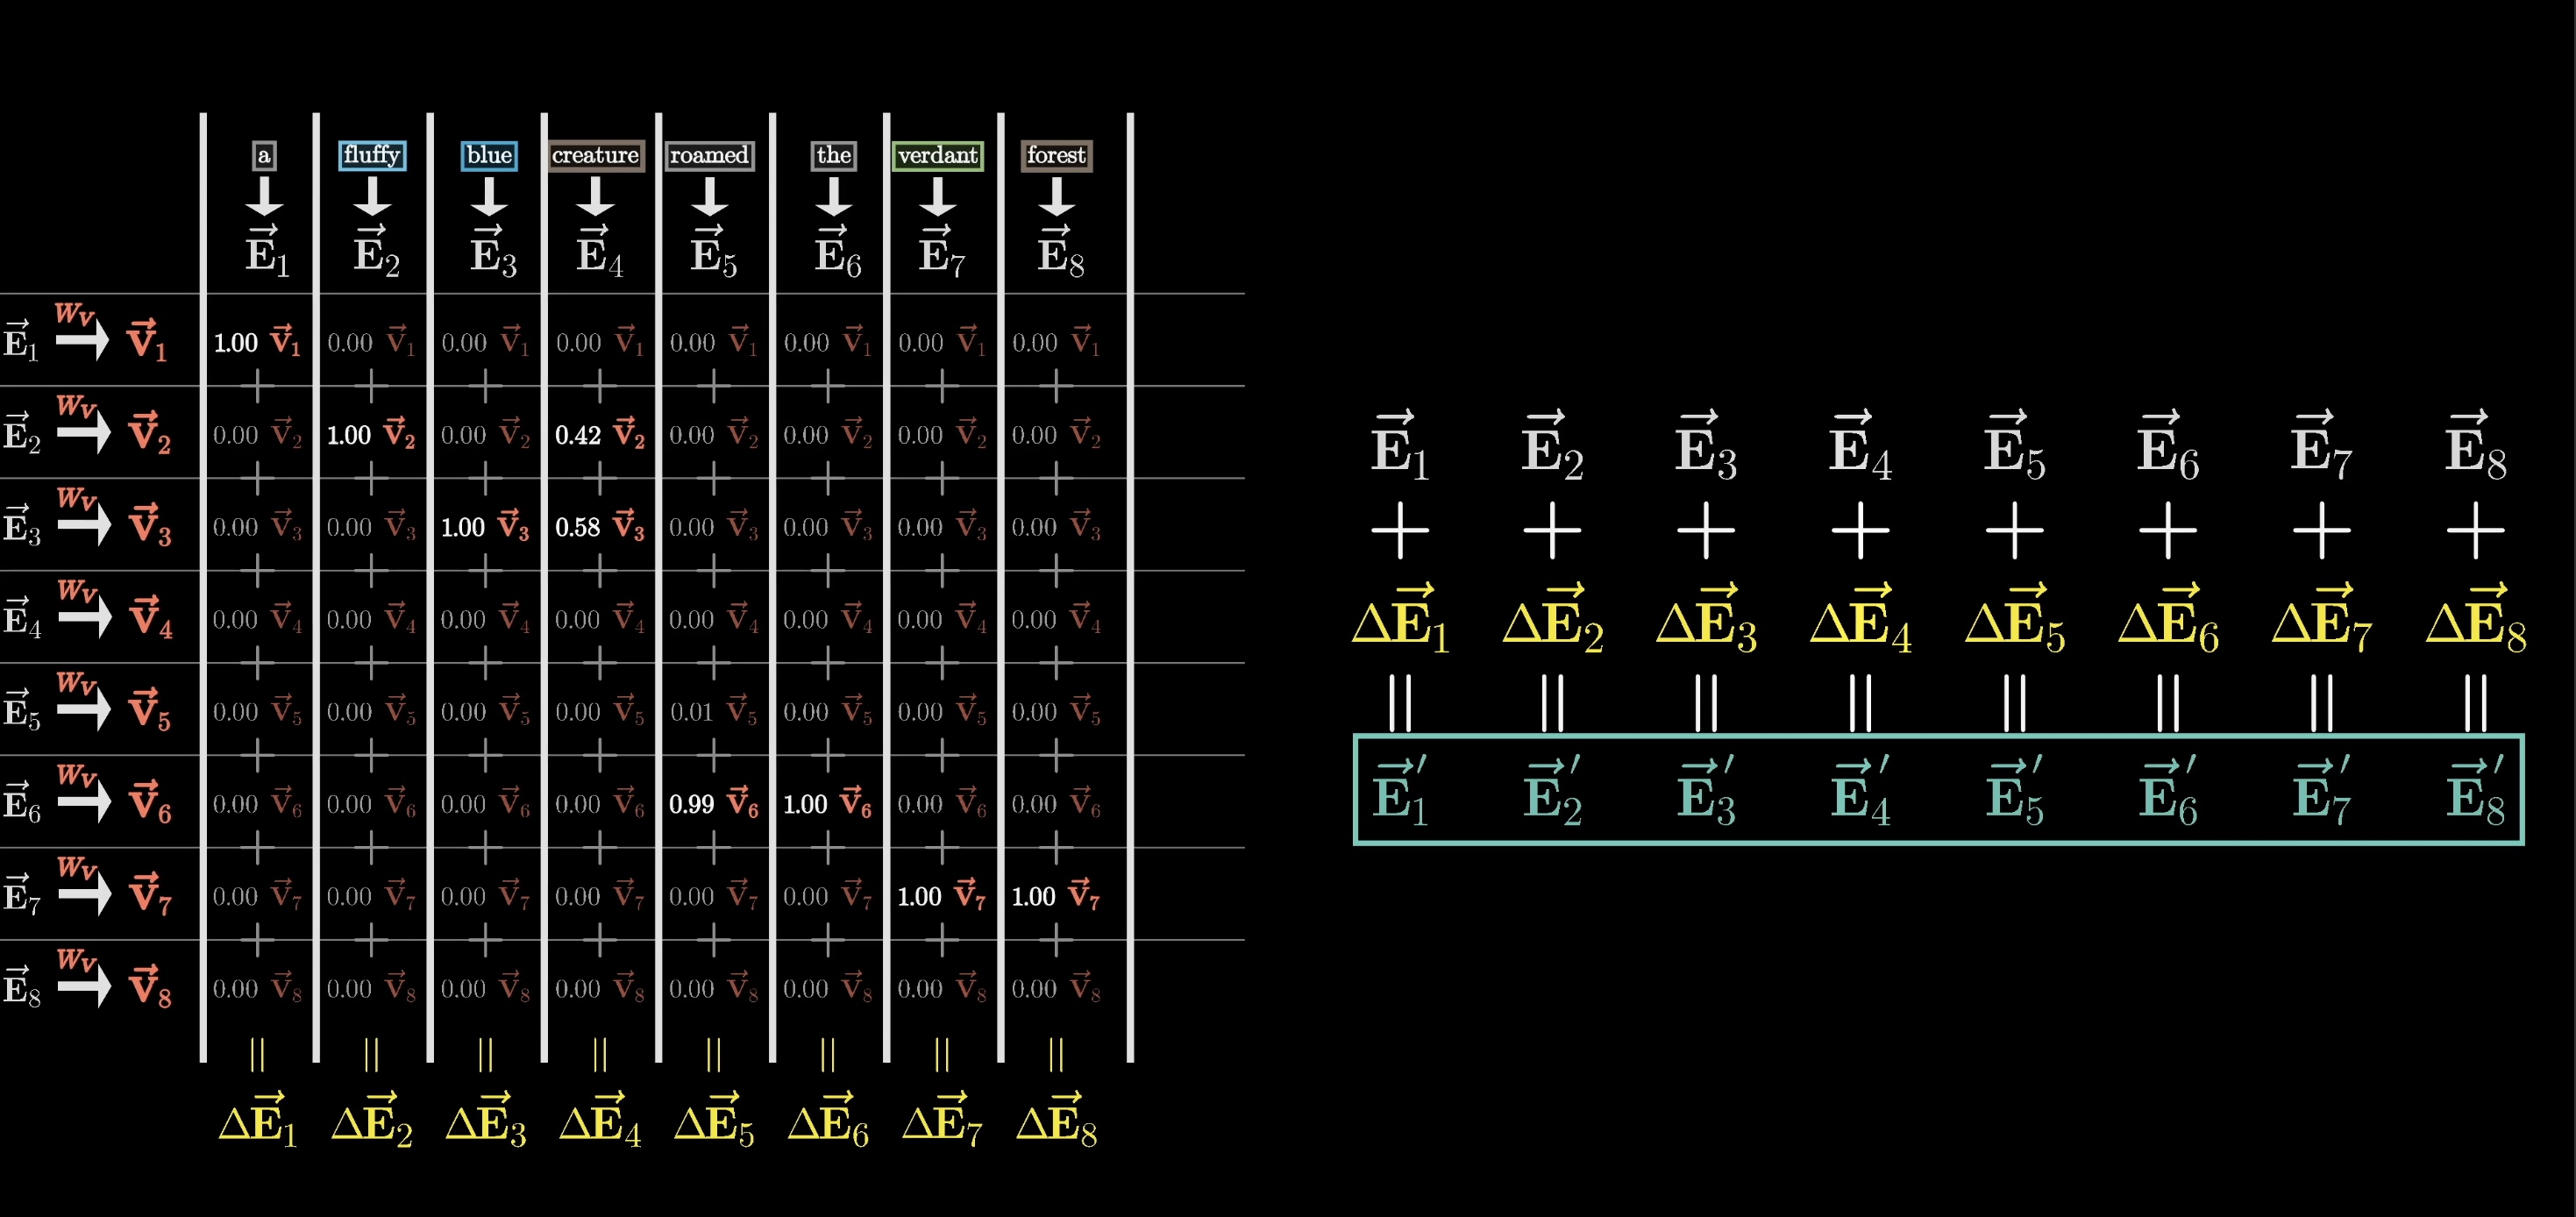
\includegraphics[height=0.72\textheight,width=0.95\linewidth,keepaspectratio]{./img/SingleHead.jpg}%
            }{%
                \fbox{\begin{minipage}[c][3cm][c]{0.9\linewidth}\centering Image \texttt{./img/SingleHead.jpg} manquante\end{minipage}}%
            }
        \end{column}
        \begin{column}{0.44\textwidth}
            Une \textbf{tête d'attention} : chaque token fabrique trois petits vecteurs (des paramètres appris) :
            \begin{itemize}\setlength\itemsep{0.3em}
                \item une \textbf{requête} : la question du type « y a-t-il un adjectif avant moi ? »
                \item une \textbf{clé} : ce que ce token peut offrir en réponse
                \item une \textbf{valeur} : l'information effectivement transmise
            \end{itemize}
        \end{column}
    \end{columns}
\end{frame}

\begin{frame}
    \frametitle{Scores de pertinence}
    \begin{columns}[c]
        \begin{column}{0.48\textwidth}
            \centering
            \IfFileExists{./img/QueryKey.jpg}{%
                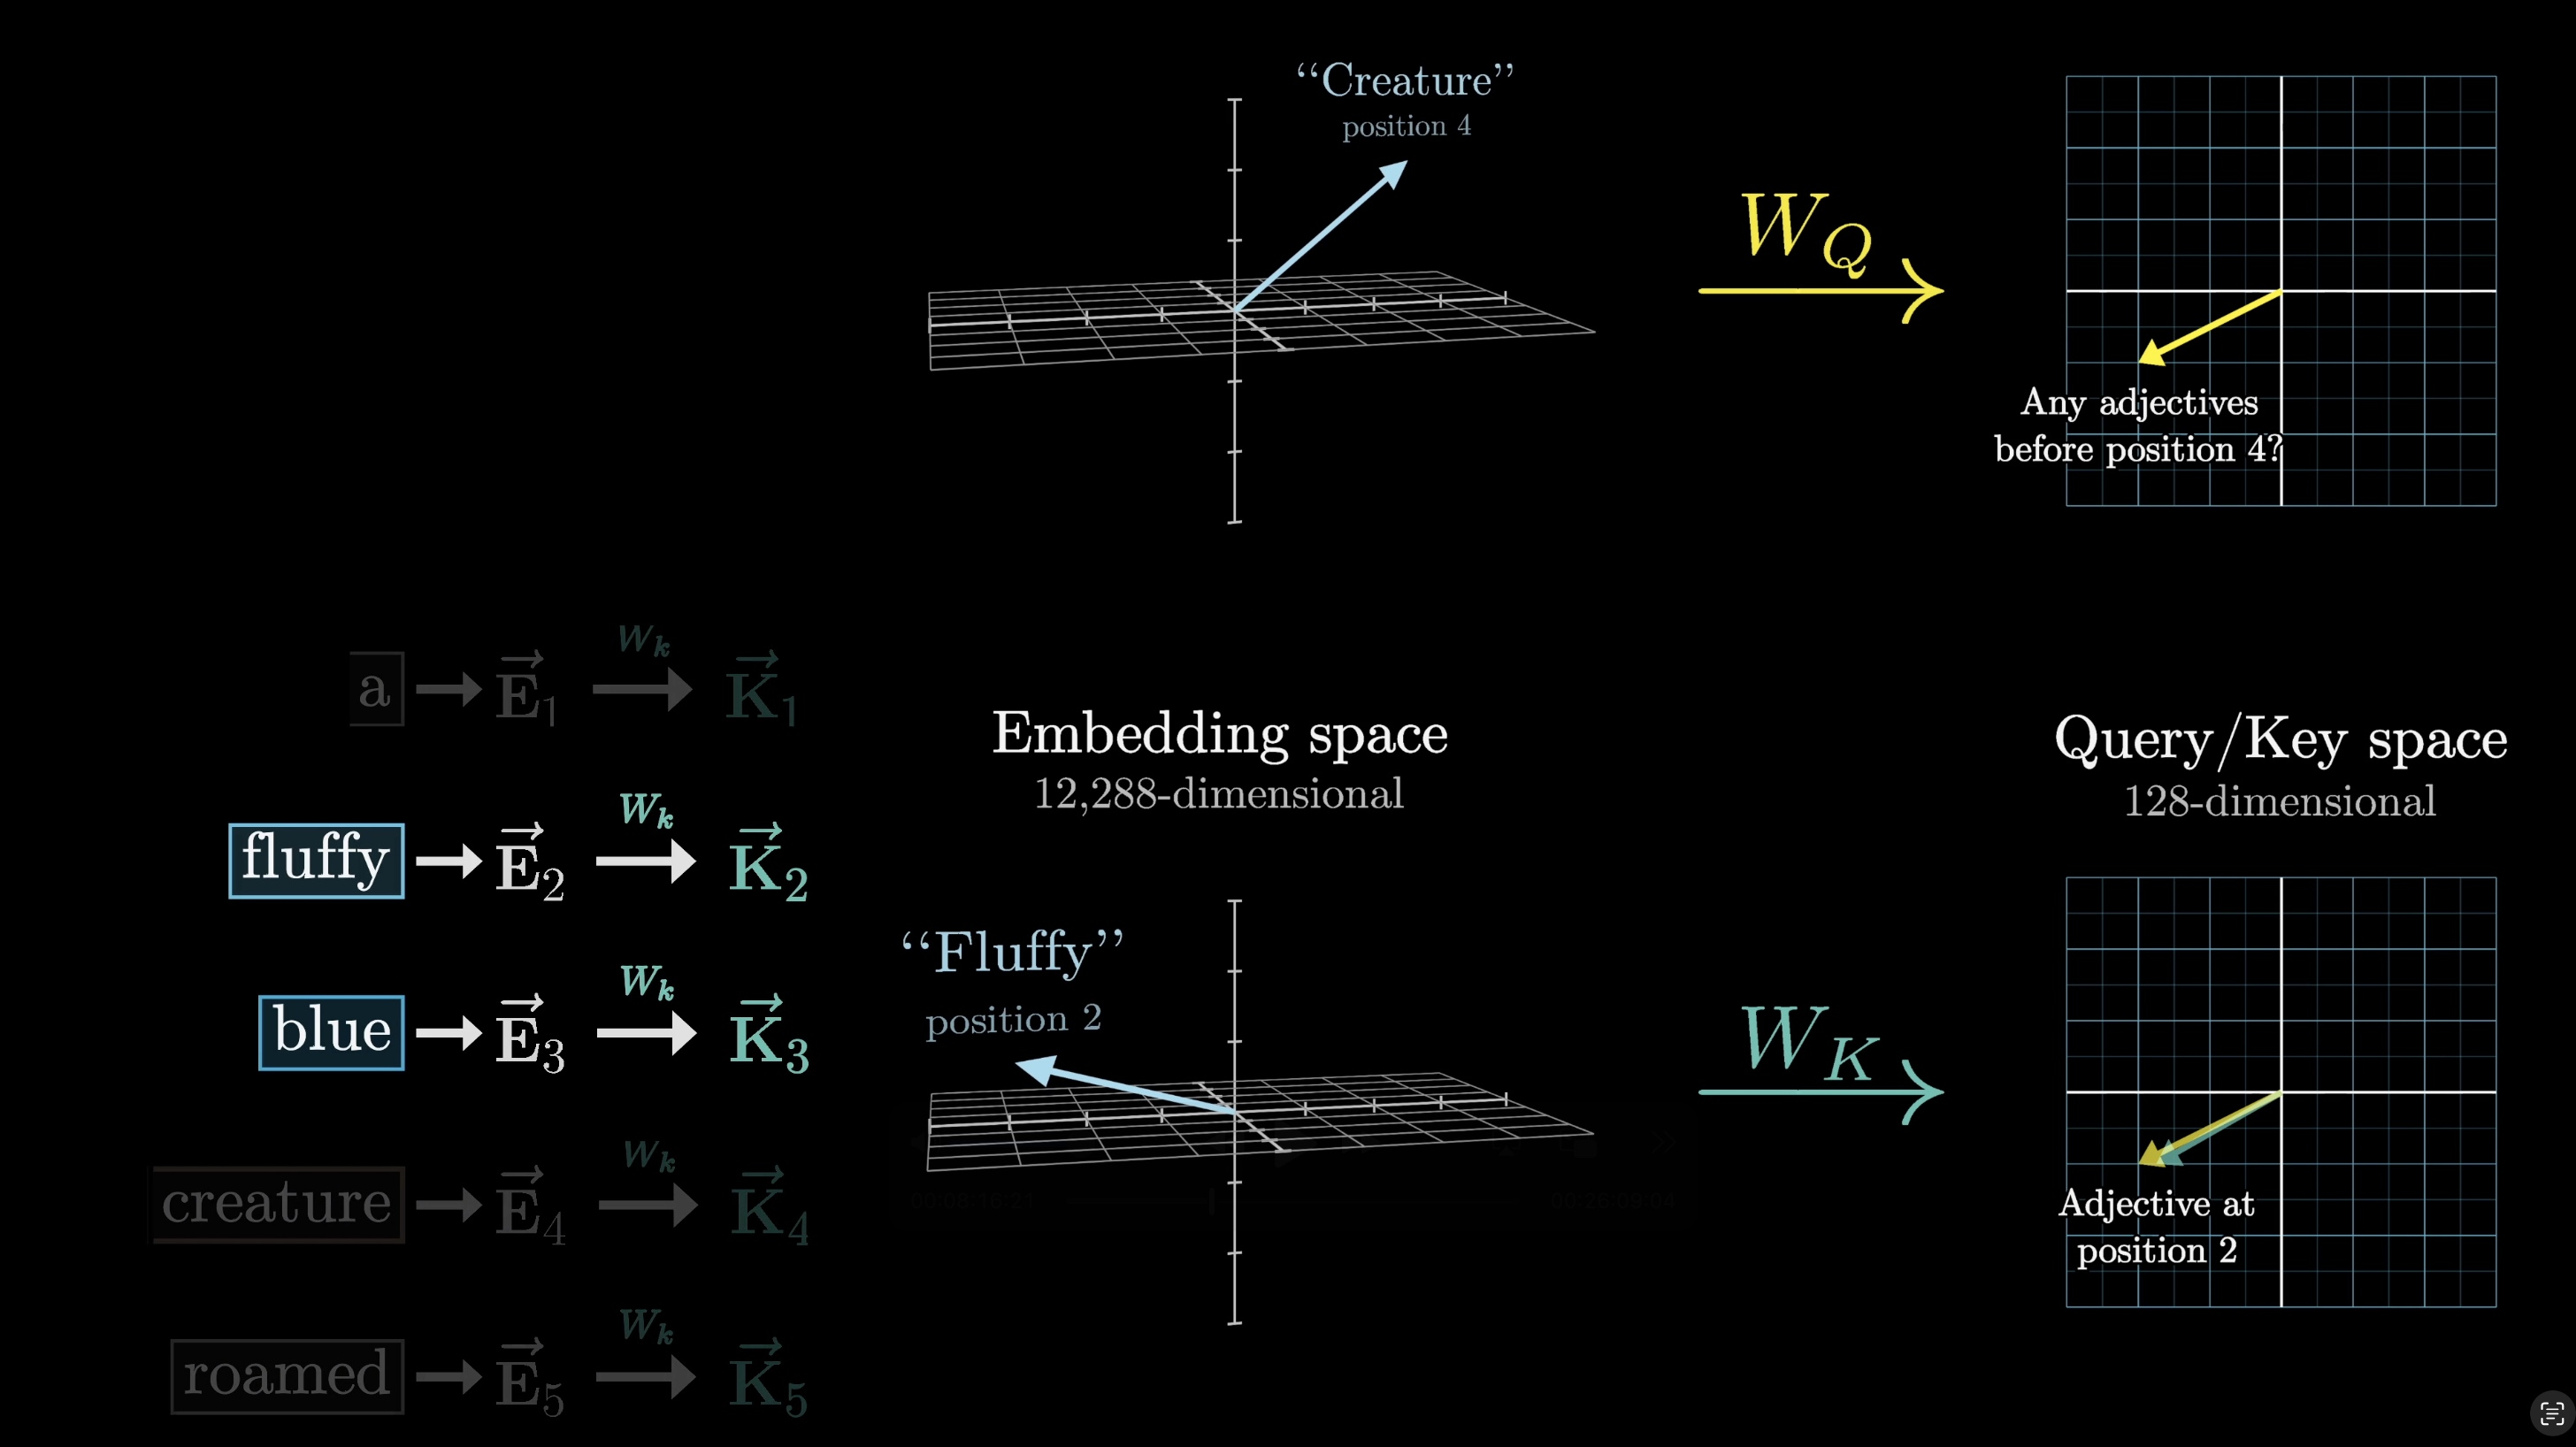
\includegraphics[height=0.55\textheight,width=0.95\linewidth,keepaspectratio]{./img/QueryKey.jpg}%
            }{%
                \fbox{\begin{minipage}[c][3cm][c]{0.9\linewidth}\centering Image \texttt{./img/QueryKey.jpg} manquante\end{minipage}}%
            }
        \end{column}
        \begin{column}{0.48\textwidth}
            \centering
            \IfFileExists{./img/DotProduct.jpg}{%
                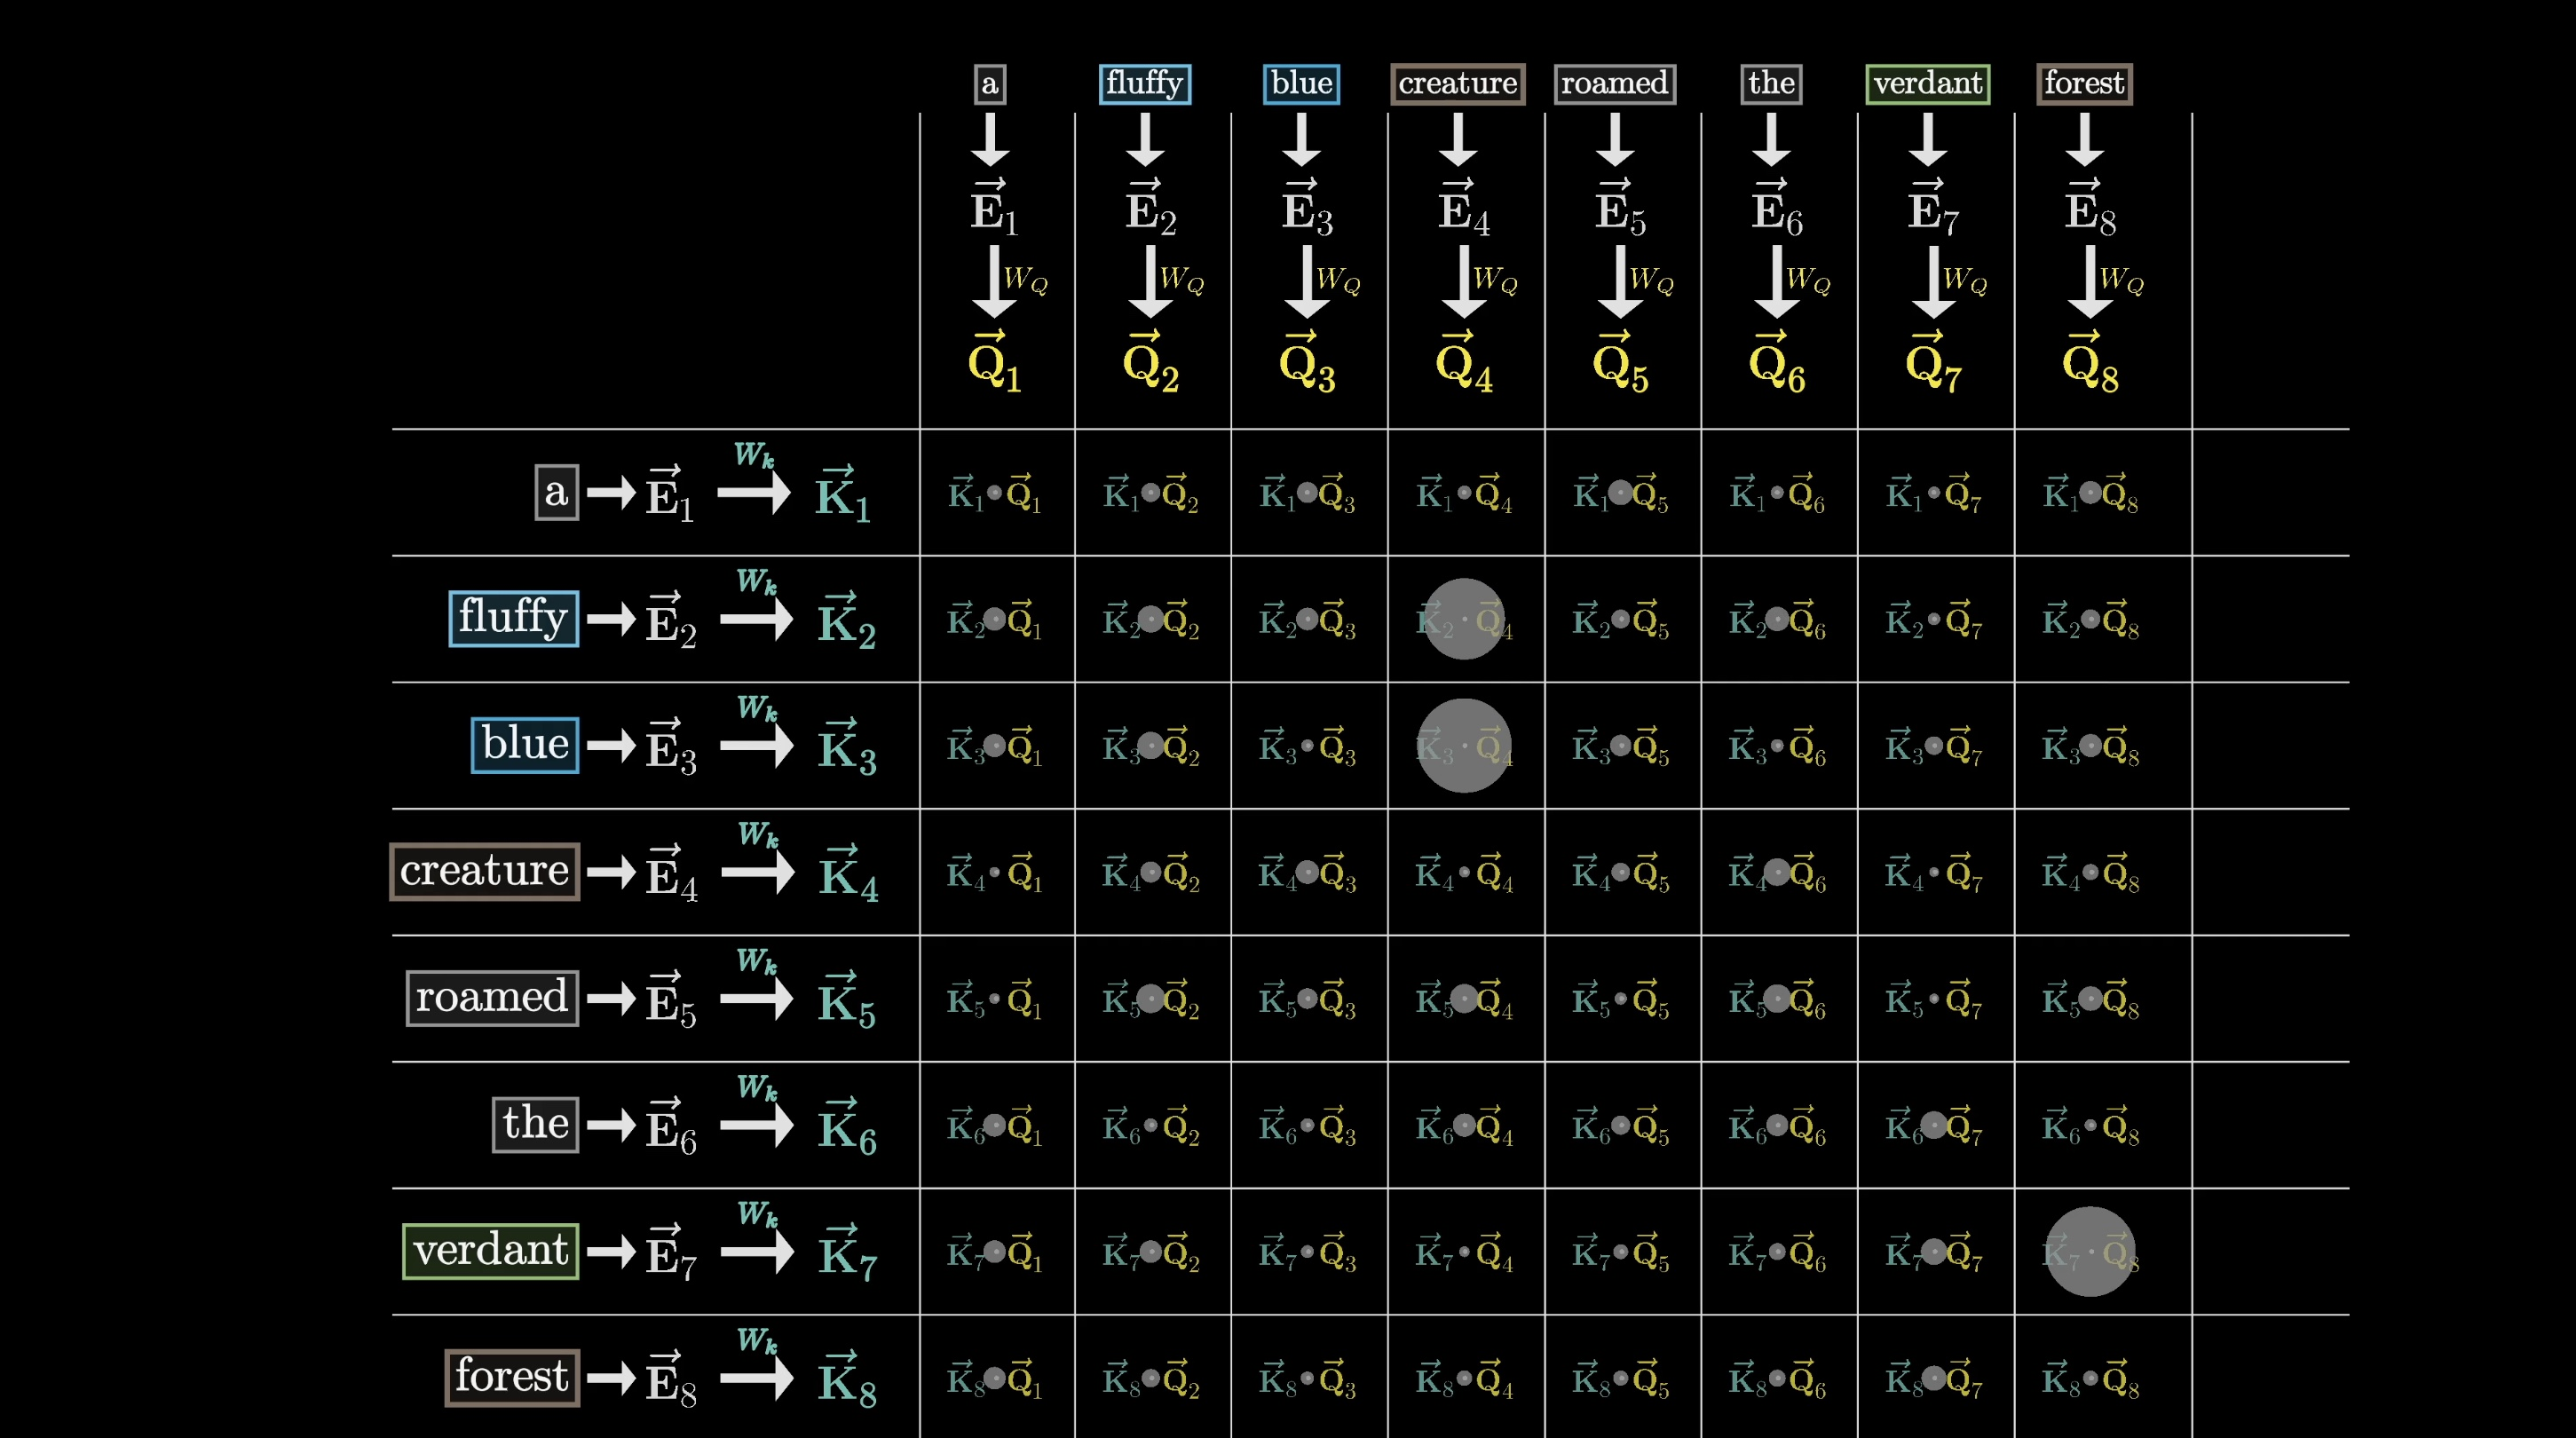
\includegraphics[height=0.55\textheight,width=0.95\linewidth,keepaspectratio]{./img/DotProduct.jpg}%
            }{%
                \fbox{\begin{minipage}[c][3cm][c]{0.9\linewidth}\centering Image \texttt{./img/DotProduct.jpg} manquante\end{minipage}}%
            }
        \end{column}
    \end{columns}
    \vspace{0.2cm}
    \begin{center}
        \small Chaque requête est comparée à chaque clé $\Rightarrow$ une grille de scores : « qui est pertinent pour mettre à jour qui ? »
    \end{center}
\end{frame}

\begin{frame}
    \frametitle{Comment un mot est mis à jour}
    \begin{columns}[c]
        \begin{column}{0.5\textwidth}
            \centering
            \IfFileExists{./img/DeltaE.jpg}{%
                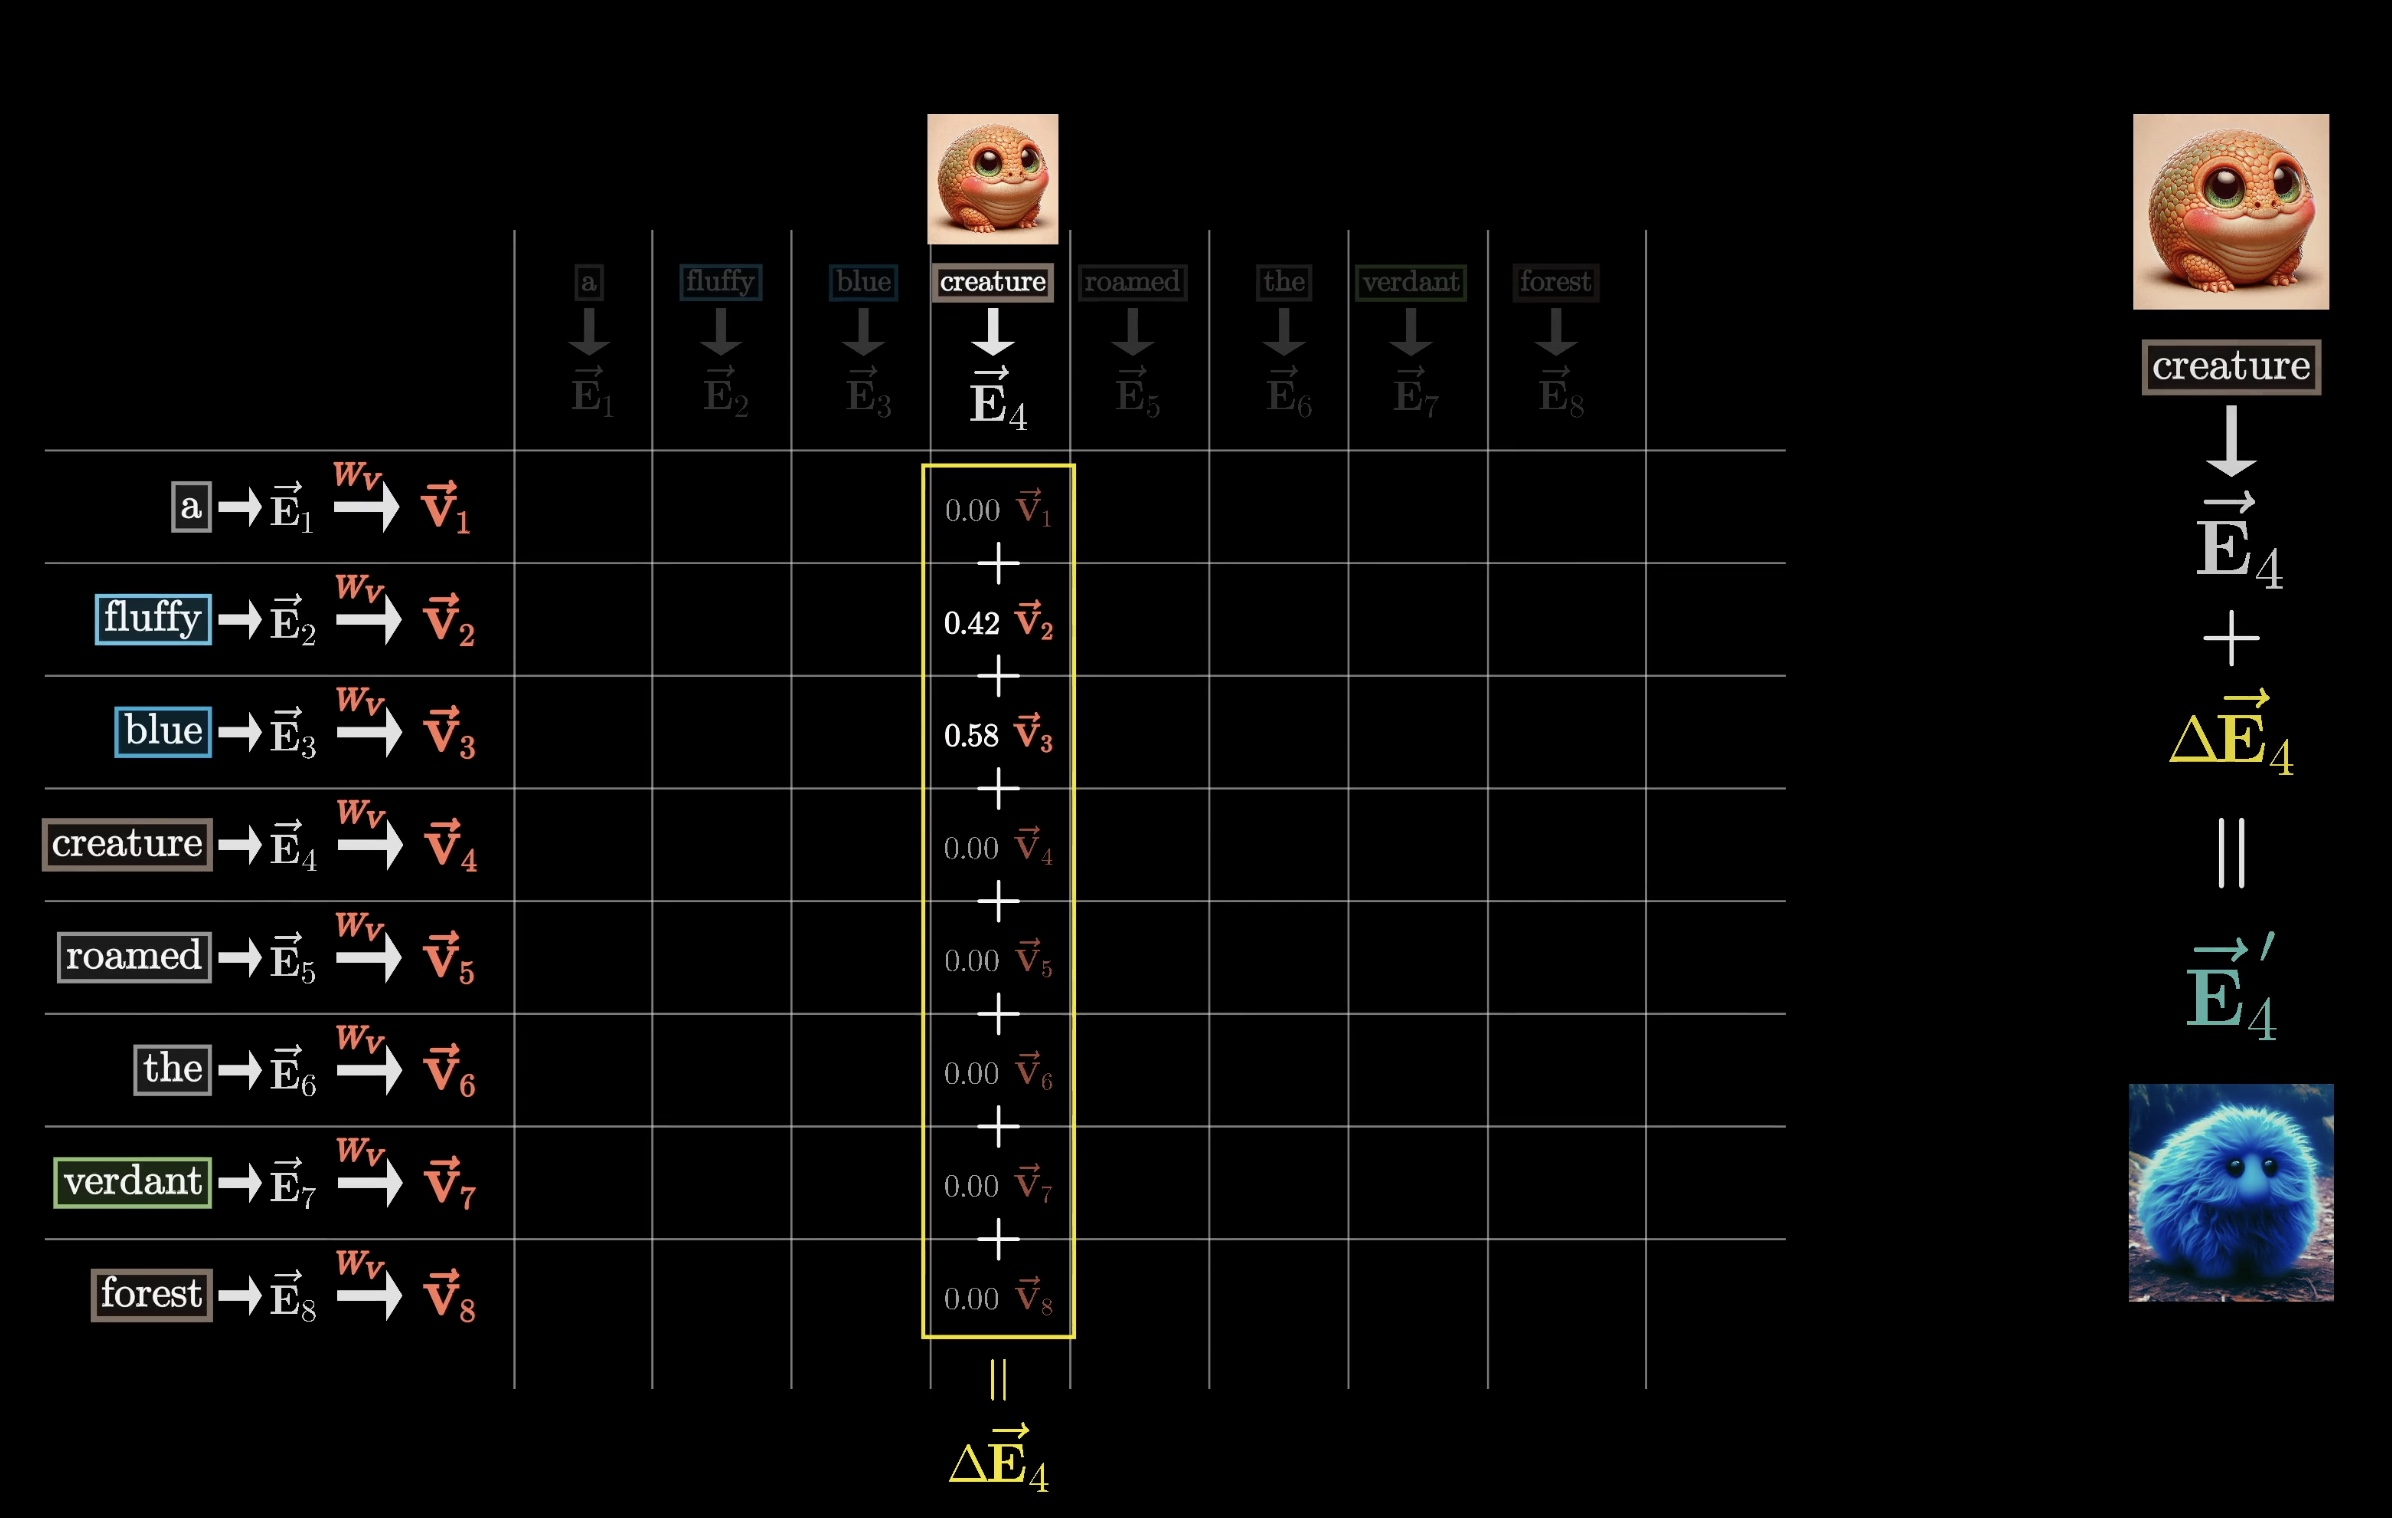
\includegraphics[height=0.62\textheight,width=0.95\linewidth,keepaspectratio]{./img/DeltaE.jpg}%
            }{%
                \fbox{\begin{minipage}[c][3cm][c]{0.9\linewidth}\centering Image \texttt{./img/DeltaE.jpg} manquante\end{minipage}}%
            }
        \end{column}
        \begin{column}{0.46\textwidth}
            Les valeurs des voisins, mélangées selon leur \textbf{pertinence}, sont \textbf{ajoutées au vecteur d'origine}.\\[0.4em]
            \emph{creature} a absorbé \emph{fluffy} et \emph{blue} $\rightarrow$ un sens contextualisé.
        \end{column}
    \end{columns}
\end{frame}

\begin{frame}
    \frametitle{Plusieurs têtes, plusieurs blocs}
    \begin{columns}[c]
        \begin{column}{0.5\textwidth}
            \centering
            \IfFileExists{./img/MultiHeaded.jpg}{%
                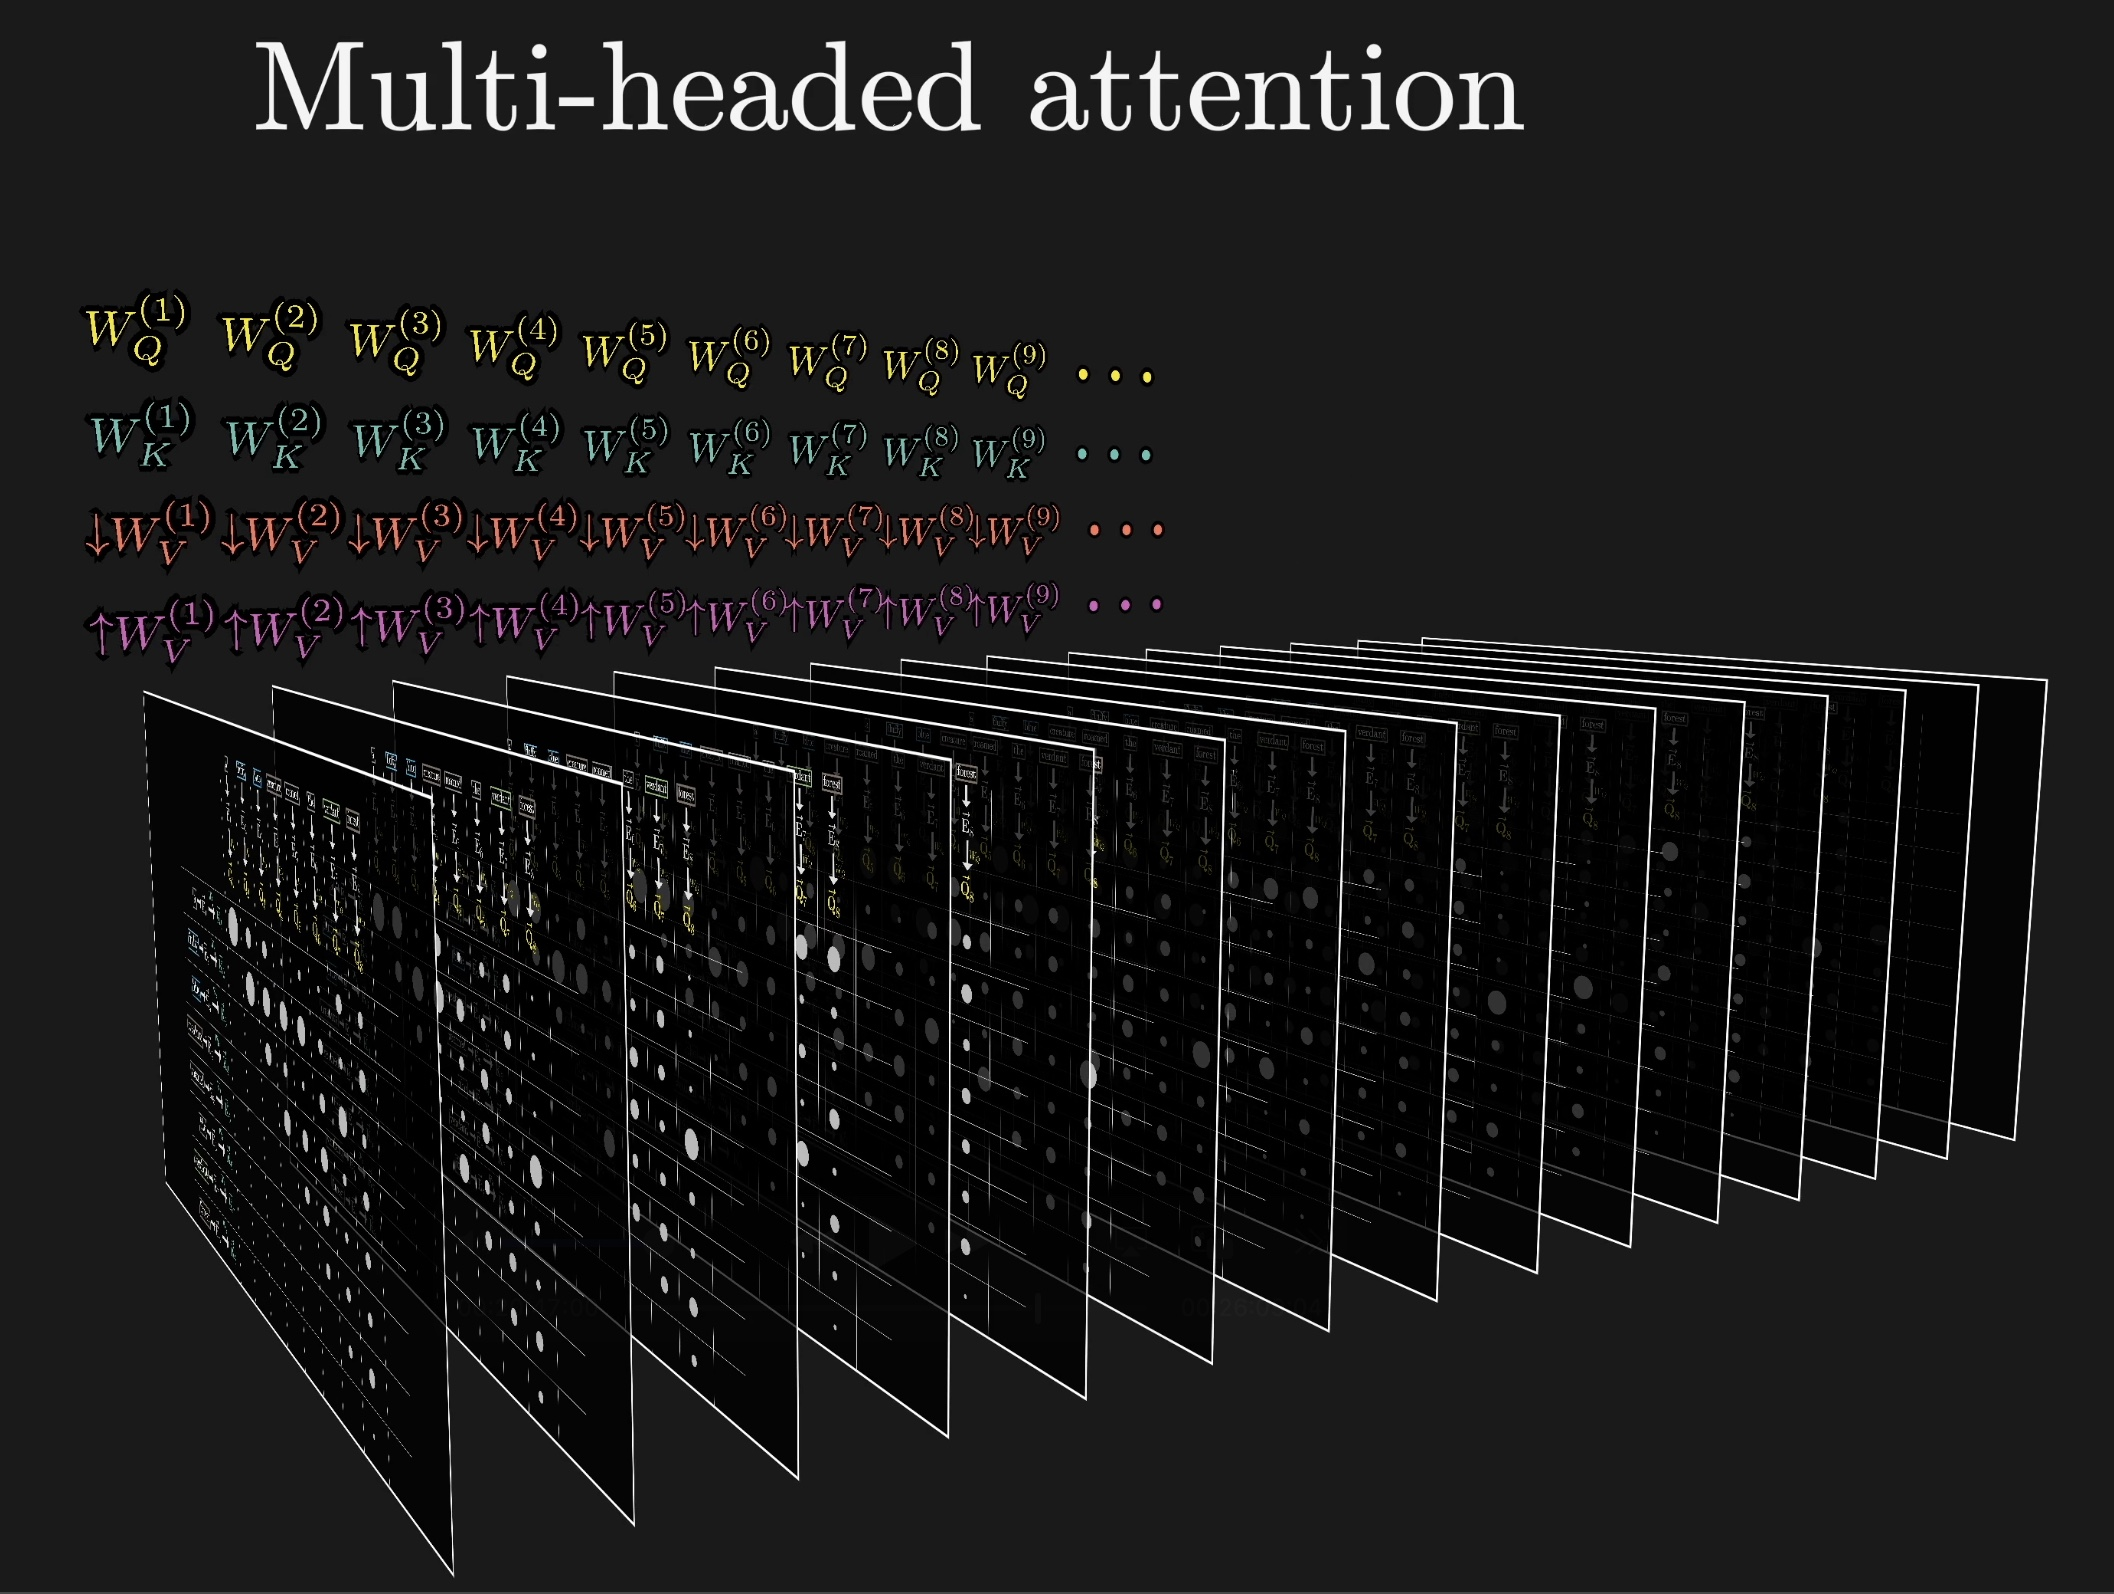
\includegraphics[height=0.6\textheight,width=0.95\linewidth,keepaspectratio]{./img/MultiHeaded.jpg}%
            }{%
                \fbox{\begin{minipage}[c][3cm][c]{0.9\linewidth}\centering Image \texttt{./img/MultiHeaded.jpg} manquante\end{minipage}}%
            }
        \end{column}
        \begin{column}{0.46\textwidth}
            \begin{itemize}\setlength\itemsep{0.4em}
                \item Une \textbf{attention multi-têtes} : des têtes parallèles, chacune ses propres paramètres $\rightarrow$ autant de « façons dont le contexte change le sens » (ex. grammaire \emph{vs} références : Harry $\rightarrow$ sorcier ou prince ?)
                \item Des \textbf{centaines de blocs} empilés (attention + MLP) : chaque passage affine les plongements --- sentiment, ton, style\dots
            \end{itemize}
        \end{column}
    \end{columns}
\end{frame}

\begin{frame}
    \frametitle{En vrai, ça compte combien de paramètres ?}
    \begin{columns}[c]
        \begin{column}{0.5\textwidth}
            \centering
            \IfFileExists{./img/FinalCount.jpg}{%
                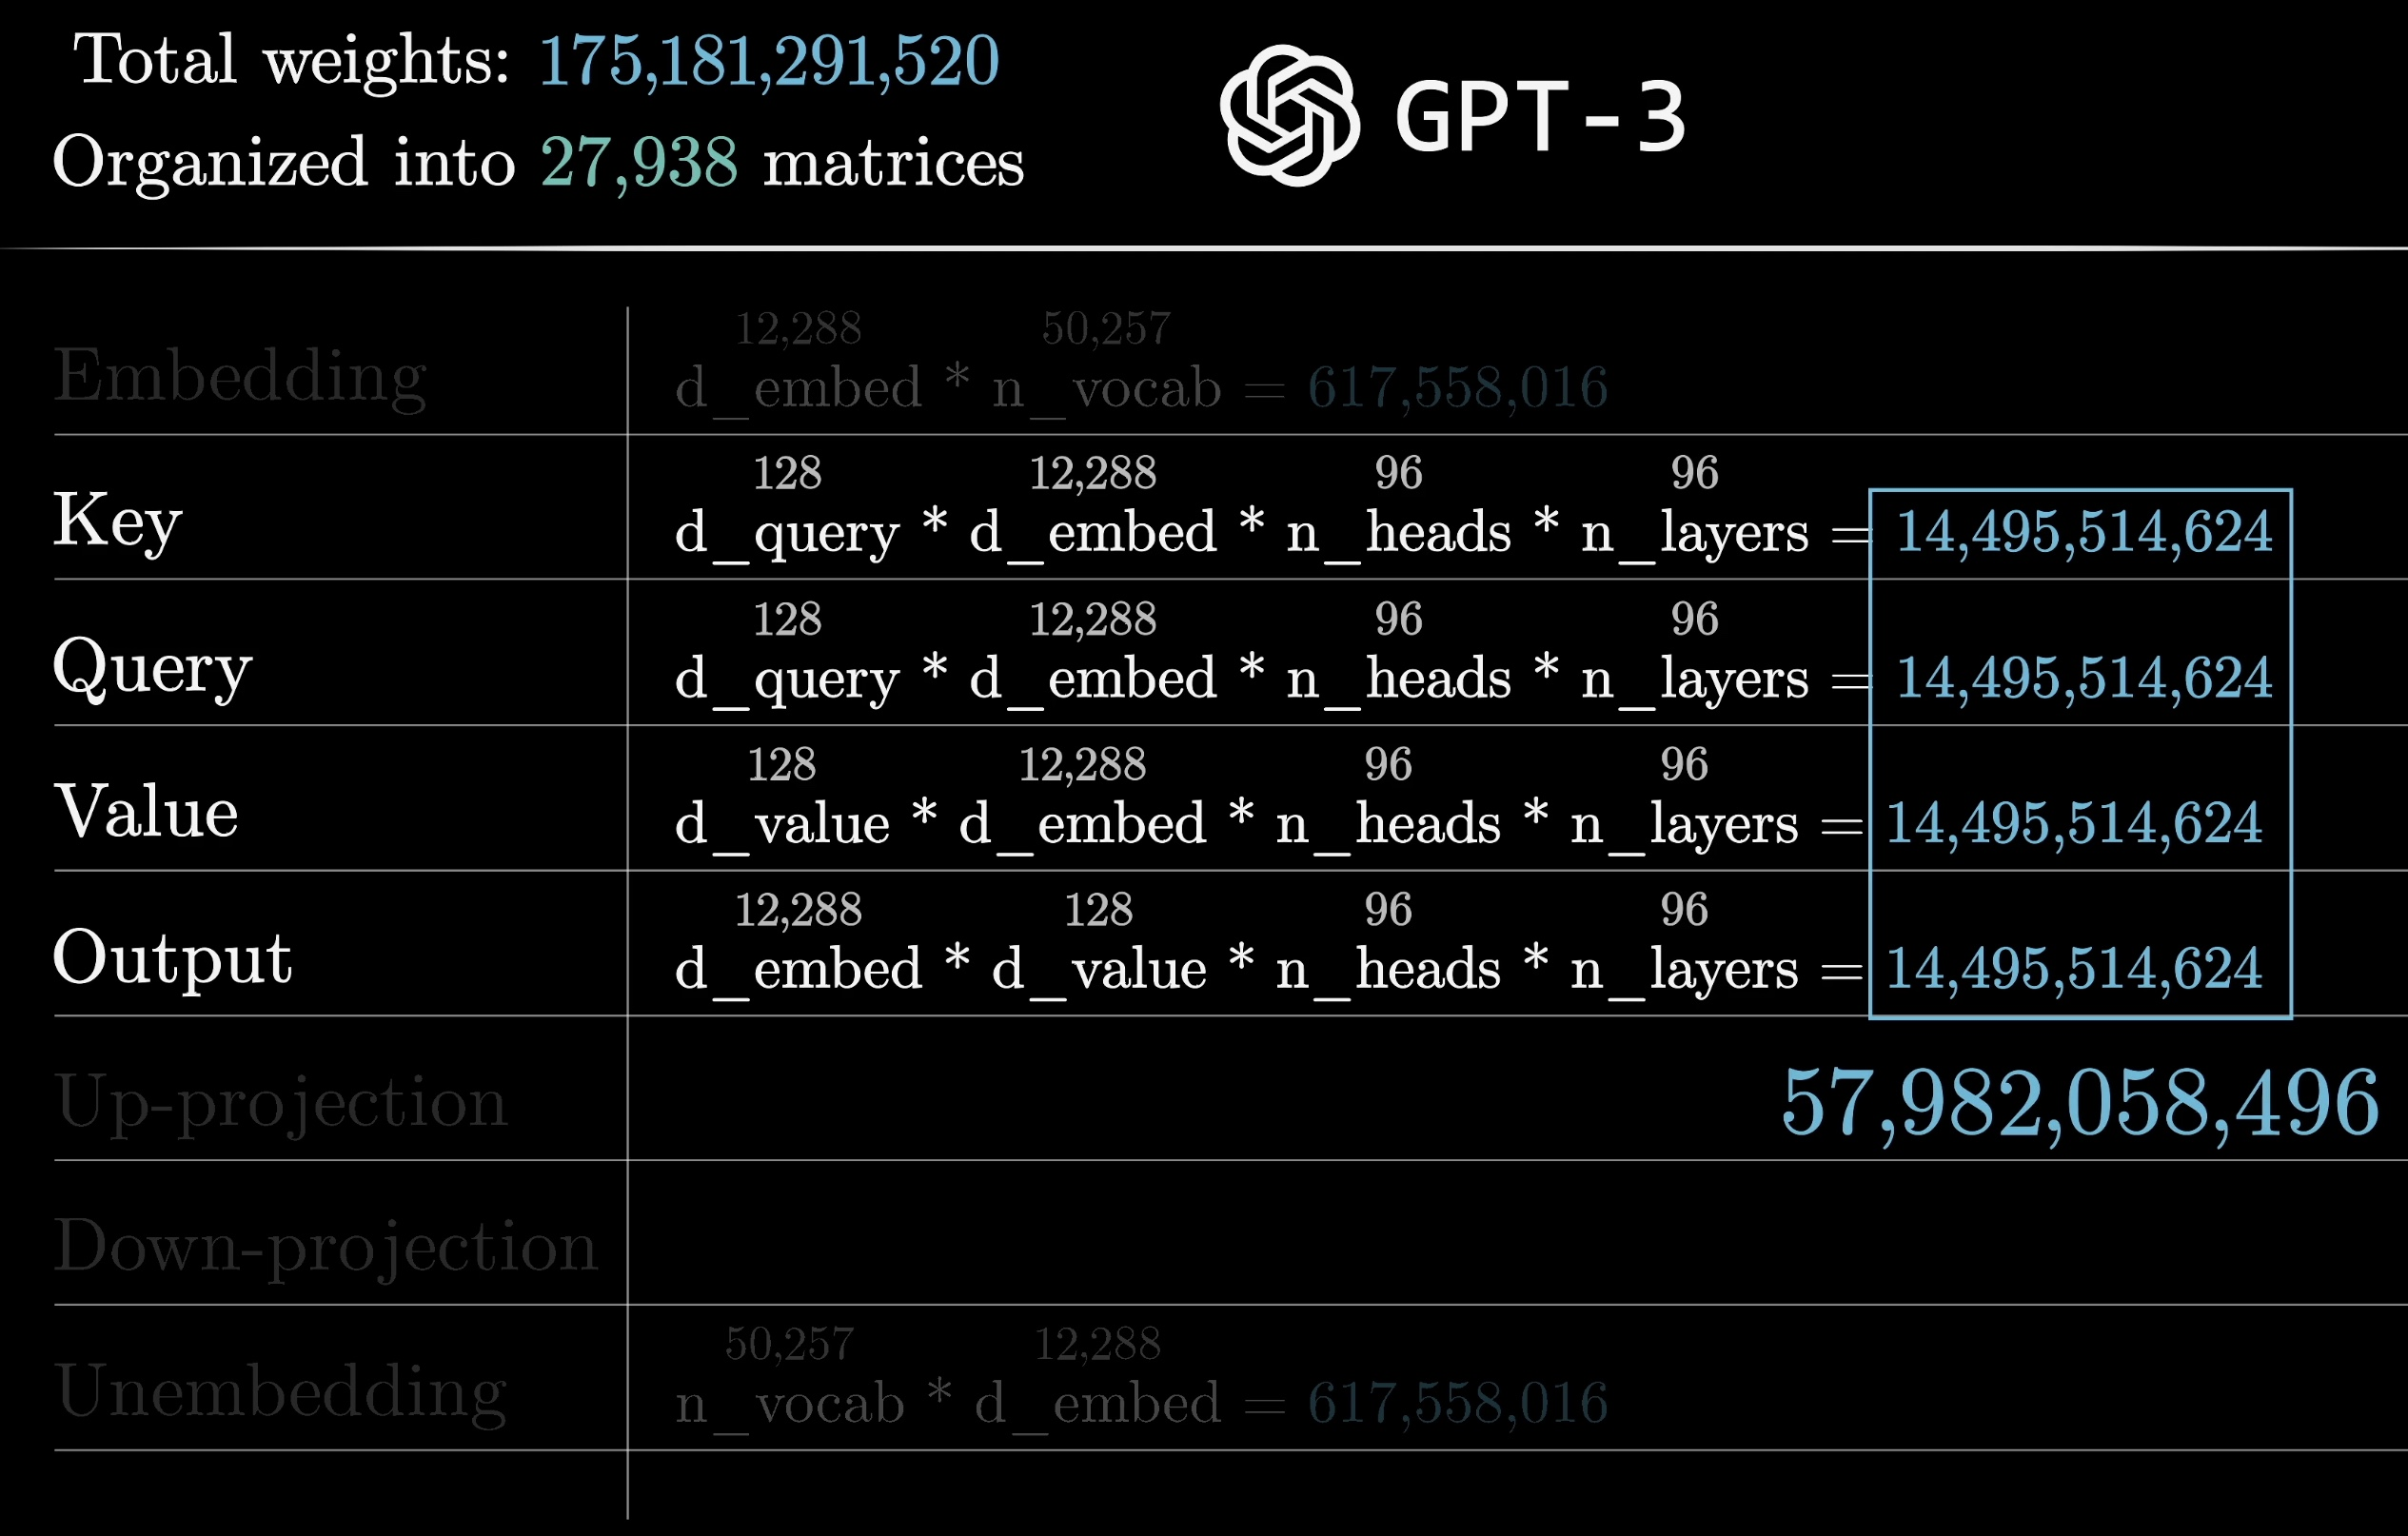
\includegraphics[height=0.62\textheight,width=0.95\linewidth,keepaspectratio]{./img/FinalCount.jpg}%
            }{%
                \fbox{\begin{minipage}[c][3cm][c]{0.9\linewidth}\centering Image \texttt{./img/FinalCount.jpg} manquante\end{minipage}}%
            }
        \end{column}
        \begin{column}{0.46\textwidth}
            Un ordre de grandeur pour donner envie :
            \begin{itemize}\setlength\itemsep{0.3em}
                \item GPT-3 : 96 couches, des dizaines de têtes chacune
                \item L'attention représente environ \textbf{un tiers des 175 milliards de paramètres}
            \end{itemize}
            \emph{Tout ça, ce sont des nombres à stocker $\Rightarrow$ pourquoi la quantification (partie 2) est indispensable.}
        \end{column}
    \end{columns}
\end{frame}

\begin{frame}
    \frametitle{Pourquoi le contexte coûte cher}
    \begin{columns}[c]
        \begin{column}{0.5\textwidth}
            \centering
            \IfFileExists{./img/square.jpg}{%
                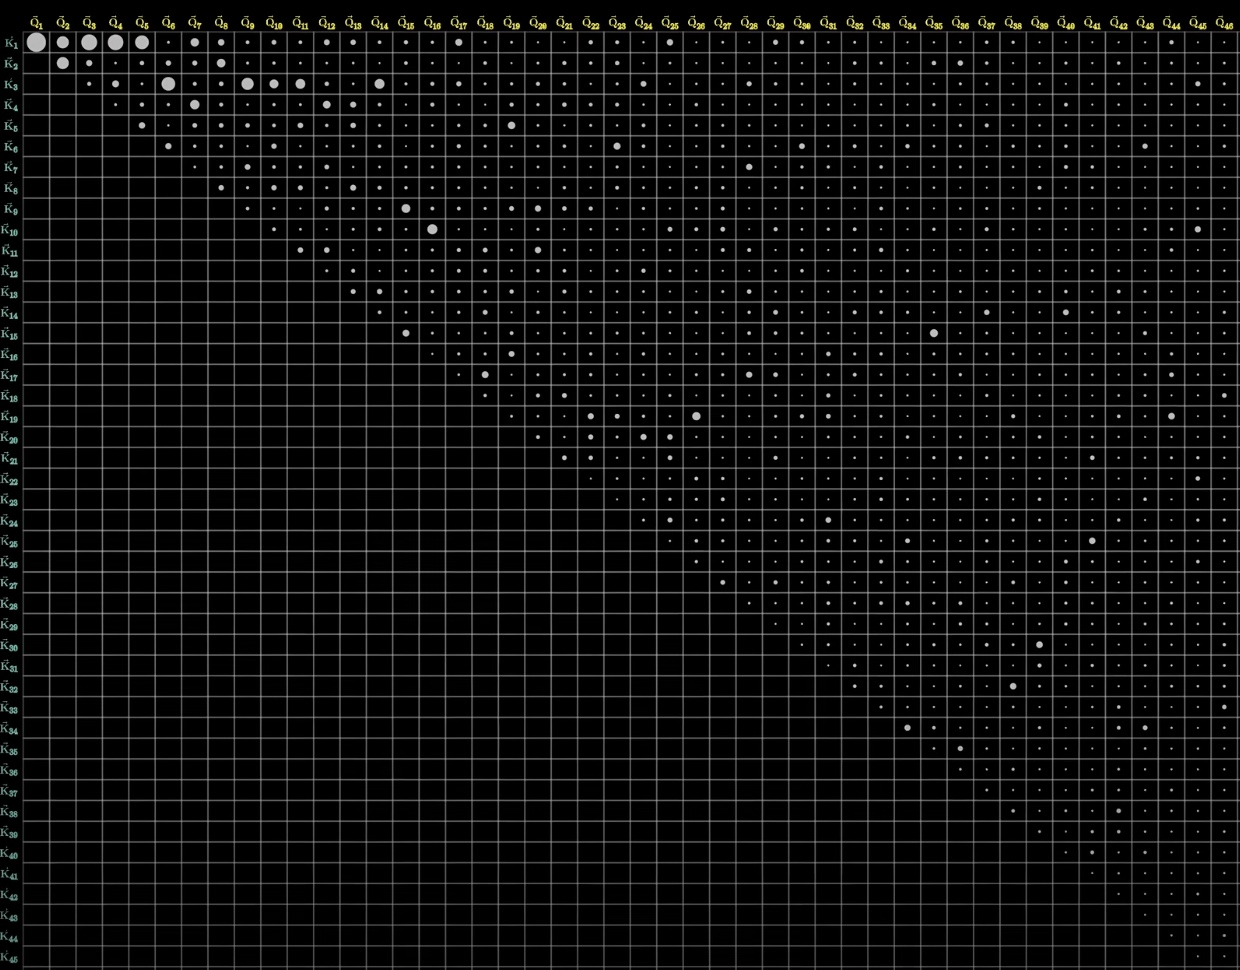
\includegraphics[height=0.66\textheight,width=0.95\linewidth,keepaspectratio]{./img/square.jpg}%
            }{%
                \fbox{\begin{minipage}[c][3cm][c]{0.9\linewidth}\centering Image \texttt{./img/square.jpg} manquante\end{minipage}}%
            }
        \end{column}
        \begin{column}{0.46\textwidth}
            \begin{itemize}\setlength\itemsep{0.4em}
                \item Chaque token peut interagir avec \emph{tous} les autres : doubler le contexte quadruple le travail
                \item En génération, on garde en mémoire les clés/valeurs de chaque token : le \textbf{KV cache}
                \item La fenêtre de contexte est donc une vraie limite \emph{physique}, pas un réglage gratuit
            \end{itemize}
        \end{column}
    \end{columns}
\end{frame}

\begin{frame}[fragile]
    \frametitle{Prefilling et décodage}
    \begin{itemize}\setlength\itemsep{0.4em}
        \item \textbf{Prefilling} : tout le prompt est traité \emph{en parallèle} (rapide, exploite le GPU) $\rightarrow$ remplit le KV cache
        \item \textbf{Décodage} : ensuite, un token à la fois (lent, limité par la mémoire) $\rightarrow$ c'est le \texttt{tok/s} affiché par llama.cpp
        \item \textbf{Échantillonnage} : la température est un dé plus ou moins pipé sur le tirage du mot suivant $\rightarrow$ déterminisme \emph{vs} créativité
    \end{itemize}
    \vfill
    \begin{lstlisting}[language=bash]
llm ... eval:  12.3 t/s decod |  1450 t/s prefill | ctx 8192
    \end{lstlisting}
    \small (les deux vitesses n'ont rien à voir --- gardez-le en tête pour les agents, partie 3)
\end{frame}

\begin{frame}
    \frametitle{Ce qu'un LLM n'est \emph{pas}}
    \begin{itemize}\setlength\itemsep{0.5em}
        \item \textbf{Pas une base de données} : « halluciner » = continuer plausiblement, pas rattraper une erreur de fait
        \item \textbf{Pas de mémoire} entre deux appels : chaque requête repart de zéro \\ $\Rightarrow$ c'est le \emph{logiciel autour} qui gère l'historique (partie 3)
        \item \textbf{Pas de compréhension symbolique certifiable} : ce qui marche remarquablement bien, avec un modèle statistique sous le capot
    \end{itemize}
    \vfill
    \begin{center}
        \begin{block}{}
            Et pourtant ça marche : l'attention est \textbf{massivement parallélisable} sur GPU, et l'échelle seule a produit des sauts qualitatifs. C'est la leçon des 10 dernières années.
        \end{block}
    \end{center}
\end{frame}

%========================================================================================
\section{Faire tourner un modèle}
%========================================================================================

\begin{frame}
    \frametitle{llama.cpp et le format GGUF}
    \begin{columns}[t]
        \begin{column}{0.55\textwidth}
            \begin{block}{\centering \textbf{llama.cpp (projet ggml)}}
                \begin{itemize}\setlength\itemsep{0.3em}
                    \item Inférence LLM en C/C++ pur, sans dépendances, MIT, $\sim$130k étoiles GitHub
                    \item « minimal setup, state-of-the-art performance on a wide range of hardware »
                    \item Backends : Metal (Apple), CUDA, Vulkan, HIP, CPU (AVX/NEON)\dots + hybride CPU+GPU
                \end{itemize}
            \end{block}
        \end{column}
        \begin{column}{0.42\textwidth}
            \begin{exampleblock}{\centering \textbf{GGUF}}
                \begin{itemize}\setlength\itemsep{0.3em}
                    \item Format conteneur : poids \emph{+} tokenizer \emph{+} gabarit de chat
                    \item Distribué sur Hugging Face
                    \item Une même famille existe en plusieurs \textbf{quantifications} --- un fichier = un choix
                \end{itemize}
            \end{exampleblock}
        \end{column}
    \end{columns}
\end{frame}

\begin{frame}
    \frametitle{La quantification}
    \begin{center}
        \footnotesize
        \begin{tabular}{@{}lll@{}}
            \toprule
            \textbf{Schéma} & \textbf{bits/poids (env.)} & \textbf{Usage} \\
            \midrule
            Q8\_0   & $\sim$8,5 & quasi sans perte, gros \\
            \textbf{Q4\_K\_M} & $\sim$4,8 & \textbf{le défaut recommandé} : l'essentiel de Q8 à mi-taille \\
            Q3\_K\_M & $\sim$3,3 & compromis serré, la qualité baisse vite \\
            Q2\_K\_S & $\sim$2,5 & dernier recours \\
            \bottomrule
        \end{tabular}
    \end{center}
    \vfill
    \begin{itemize}\setlength\itemsep{0.4em}
        \item Le modèle stocke des nombres à 16 bits ; les compresser à 4--5 bits divise la mémoire par 3--4 avec peu de perte perceptible
        \item Les repos « Dynamic GGUF » (Unsloth) optimisent le choix couche par couche
    \end{itemize}
\end{frame}

\begin{frame}
    \frametitle{Dimensionner : poids + KV cache}
    \begin{center}
        {\large \textbf{poids} ($\approx$ \#paramètres $\times$ bits/poids) \ \textbf{+ KV cache} (contexte) \ $\leq$ \textbf{RAM/VRAM}}
    \end{center}
    \bigskip
    \begin{center}
        \begin{tabular}{@{}llll@{}}
            \toprule
            \textbf{Modèle} & \textbf{Quant.} & \textbf{Poids} & \textbf{Machine type} \\
            \midrule
            0{,}8B & Q4\_K\_M & $\sim$0{,}5 Go & n'importe quel laptop \\
            4--8B & Q4\_K\_M & $\sim$2{,}5--5 Go & laptop récent / GPU 6--8 Go \\
            9--14B & Q4\_K\_M & $\sim$5--9 Go & GPU 12 Go \\
            35B & Q4\_K\_M & $\sim$21 Go (avec ctx 32k) & RTX 3090/4090 \\
            \bottomrule
        \end{tabular}
    \end{center}
    \vfill
    \begin{alertblock}{}
        Le KV cache s'ajoute au-dessus, et il grandit avec le contexte. Un agent construit des prompts longs : prévoyez large (cf. exercice).
    \end{alertblock}
\end{frame}

\begin{frame}
    \frametitle{Le paysage des modèles (sept. 2026)}
    \begin{itemize}\setlength\itemsep{0.5em}
        \item \textbf{Qwen3.5} (0{,}8B $\rightarrow$ 35B+), \textbf{Qwen3.8-Flash-Next}, \textbf{Gemma 4} (variantes QAT), gpt-oss\dots --- le paysage bouge \emph{vraiment} vite
        \item Les modèles MoE (experts épars) : efficaces mais gourmands --- experts déchargés sur disque = lent
        \item Règle pratique : prendre la \textbf{plus grande famille que votre machine accepte en Q4}, en instruct (pas « thinking » par défaut pour les agents)
        \item Où chercher : Hugging Face, dépôts Unsloth ; docs llama.cpp pour les archis supportées
    \end{itemize}
    \vfill
    \small (vérifié le 29/09/2026 --- relire la liste « vérifier la veille » du plan le jour J)
\end{frame}

\begin{frame}[fragile]
    \frametitle{Trois commandes suffisent}
    \begin{enumerate}
        \item \textbf{Discuter dans le terminal} (télécharge depuis Hugging Face) :
\begin{lstlisting}[language=bash]
llama cli -hf ggml-org/Qwen3.5-0.8B-GGUF
\end{lstlisting}
        \item \textbf{Servir le modèle} (API compatible OpenAI \emph{et} interface web intégrée) :
\begin{lstlisting}[language=bash]
llama-server -hf ggml-org/Qwen3.5-0.8B-GGUF \
  --host 127.0.0.1 --port 8080 -c 8192 --jinja
\end{lstlisting}
        \item \textbf{Comprendre la ligne d'état} : \texttt{prefill} $\gg$ \texttt{decode} en tok/s ; \texttt{-c} = taille du contexte $\Rightarrow$ KV cache.
    \end{enumerate}
    \vfill
    \begin{alertblock}{}
        \texttt{-\/-jinja} active le gabarit de chat natif du modèle --- indispensable pour que les appels d'outils (partie 3) sortent au format OpenAI. Sans lui, un agent reste un chatbot.
    \end{alertblock}
\end{frame}

\begin{frame}[fragile]
    \frametitle{\normalsize\bfseries Démo A --- un modèle qui tourne chez vous (en direct)}
    \begin{columns}[t]
        \begin{column}{0.5\textwidth}
            \begin{block}{\footnotesize Script}
\begin{lstlisting}[language=bash, basicstyle=\ttfamily\scriptsize]
# 1. chat terminal
llama cli -hf ggml-org/Qwen3.5-0.8B-GGUF

# 2. serveur + web UI
llama-server -hf ggml-org/Qwen3.5-0.8B-GGUF \
  --host 127.0.0.1 --port 8080 \
  -c 8192 --jinja
# puis: http://127.0.0.1:8080
\end{lstlisting}
            \end{block}
        \end{column}
        \begin{column}{0.46\textwidth}
            \begin{exampleblock}{\footnotesize À regarder}
                \begin{itemize}\setlength\itemsep{0.3em}
                    \item le téléchargement et la taille du fichier GGUF
                    \item la ligne \texttt{tok/s} : préfilling vs décodage
                    \item même question en Q4 puis Q8 : taille vs qualité
                    \item l'API : \texttt{GET /v1/models}
                \end{itemize}
            \end{exampleblock}
        \end{column}
    \end{columns}
    \vfill
    \small Script complet : \texttt{demo/demo\_llama.sh} (pré-télécharger les GGUF hors salle !)
\end{frame}

%========================================================================================
\section{Harnais d'agents}
%========================================================================================

\begin{frame}
    \frametitle{Chat et agent : la boucle}
    \begin{columns}[c]
        \begin{column}{0.44\textwidth}
            \centering
            \begin{tikzpicture}
                \node[box] (u) {utilisateur};
                \node[box, right=0.5cm of u] (m) {LLM};
                \draw[arr] (u) -- (m);
                \draw[arr] (m.west) -- ++(0,-0.7) -| (u);
            \end{tikzpicture}
            \small Chat : une requête $\rightarrow$ une réponse
        \end{column}
        \begin{column}{0.52\textwidth}
            \centering
            \begin{tikzpicture}
                \node[hbox] (r) {Réfléchir};
                \node[box, below right=0.5cm and 0.9cm of r] (a) {Agir \\ \scriptsize (appel d'outil)};
                \node[box, below left=0.5cm and 0.9cm of r] (o) {Observer \\ \scriptsize (résultat)};
                \draw[arr] (r) -- (a);
                \draw[arr] (a) |- (o);
                \draw[arr] (o) -- (r);
            \end{tikzpicture}
            \small Agent : boucle \emph{raisonner $\rightarrow$ agir $\rightarrow$ observer} (idée « ReAct », 2023), jusqu'à ce que la tâche soit finie
        \end{column}
    \end{columns}
    \vfill
    \begin{center}
        Un LLM seul ne peut que produire du texte. \textbf{Le harnais exécute} ses intentions.
    \end{center}
\end{frame}

\begin{frame}[fragile]
    \frametitle{L'appel d'outils (function calling)}
    \begin{enumerate}\setlength\itemsep{0.4em}
        \item Le serveur publie le \textbf{catalogue d'outils} (schémas JSON) : lire un fichier, chercher, exécuter\dots
        \item Le modèle \emph{émet} un appel structuré --- ce n'est pas lui qui l'exécute :
\begin{lstlisting}[language=bash]
tool_calls: [{"function": {"name": "read_file",
             "arguments": "{\"path\": \"parts.csv\"}"}}]
\end{lstlisting}
        \item Le harnais exécute, renvoie le résultat, la boucle continue.
    \end{enumerate}
    \vfill
    \begin{alertblock}{}
        Côté runner, il faut que le serveur sache sérialiser ces appels : llama.cpp $\rightarrow$ \texttt{-\/-jinja}. C'est le pont entre la partie 2 et la partie 3.
    \end{alertblock}
\end{frame}

\begin{frame}
    \frametitle{Un harnais, concrètement, ça fait quoi ?}
    \begin{center}
        {\large \texttt{agent = modèle + harnais}}
    \end{center}
    \bigskip
    \begin{columns}[t]
        \begin{column}{0.48\textwidth}
            \begin{block}{\centering \textbf{Le harnais gère}}
                \begin{itemize}\setlength\itemsep{0.3em}
                    \item la boucle et l'état (le modèle est sans mémoire)
                    \item l'exécution des outils, le sandbox
                    \item la gestion du contexte (fenêtre, compression)
                    \item les garde-fous : permissions, approbations
                \end{itemize}
            \end{block}
        \end{column}
        \begin{column}{0.48\textwidth}
            \begin{exampleblock}{\centering \textbf{Exemples courants}}
                \begin{itemize}\setlength\itemsep{0.3em}
                    \item Claude Code, Codex, Cursor (codage)
                    \item \textbf{DeepSeek Harness (dsh)}
                    \item harnais « interne » (livré) vs « externe » (AGENTS.md, serveurs MCP, skills --- Böckeler)
                \end{itemize}
            \end{exampleblock}
        \end{column}
    \end{columns}
\end{frame}

\begin{frame}
    \frametitle{Le coût du contexte}
    \begin{itemize}\setlength\itemsep{0.5em}
        \item Chaque requête repart avec : instructions système + catalogue d'outils + historique $\Rightarrow$ une tâche minuscule peut coûter \textbf{14{,}7K tokens d'entrée} (\textasciitilde25 schémas d'outils renvoyés à chaque étape --- mesures 08/2026)
        \item En local, ce coût se paie en \textbf{temps de préfilling}, pas en euros
        \item Piège classique : le \texttt{contextWindow} déclaré au harnais doit correspondre au \texttt{-c} du serveur \\ $\Rightarrow$ sinon \textbf{troncature silencieuse} du milieu du prompt (ou erreur franche selon l'archi)
        \item Les harnais mûrs \textbf{compriment} l'historique et mettent le contexte en cache --- comme le présent support a été rédigé par une session d'agent
    \end{itemize}
\end{frame}

\begin{frame}
    \frametitle{MCP, skills, fichiers d'instructions}
    \begin{itemize}\setlength\itemsep{0.5em}
        \item \textbf{MCP} (Model Context Protocol) : prise standardisée pour brancher des outils tiers sur n'importe quel harnais compatible
        \item \textbf{Skills} : dossiers \texttt{SKILL.md} découverts par le harnais --- procédures réutilisables, en texte pur, versionnables avec Git
        \item \textbf{AGENTS.md} : le mode d'emploi du projet, lu par l'agent avant d'agir (un « guide » --- à distinguer des « capteurs » : tests, linters, qui vérifient après)
        \item Idée commune : tout est \textbf{fichier local, lisible, versionnable} --- pas de magie
    \end{itemize}
\end{frame}

\begin{frame}[fragile]
    \frametitle{DeepSeek Harness (\texttt{dsh})}
    \begin{columns}[t]
        \begin{column}{0.52\textwidth}
            \begin{block}{\centering \textbf{Ce que c'est}}
                \begin{itemize}\setlength\itemsep{0.3em}
                    \item harnais d'agents open source (MIT, DeepSeek AI, 2026 --- « developer preview »)
                    \item architecture « tout est un plugin » (modèles, outils, UI)
                    \item Web UI locale : \texttt{npx @deepseek-ai/dsh web} $\rightarrow$ \texttt{127.0.0.1:3080}
                \end{itemize}
            \end{block}
        \end{column}
        \begin{column}{0.44\textwidth}
            \begin{exampleblock}{\centering \textbf{Brancher un modèle local}}
                \begin{itemize}\setlength\itemsep{0.3em}
                    \item Settings $\rightarrow$ Models $\rightarrow$ « Add a custom model API »
                    \item protocole \texttt{openai-completions}, base \texttt{http://127.0.0.1:8080/v1}
                    \item clé factice acceptée \emph{mais obligatoire} ; id exact du modèle ; \texttt{contextWindow} $\leq$ \texttt{-c}
                \end{itemize}
            \end{exampleblock}
        \end{column}
    \end{columns}
    \vfill
    \small Config fichier équivalente : profil \texttt{cordis.patch.yml} (voir \texttt{demo/dsh-provider-example.yaml})
\end{frame}

\begin{frame}[fragile]
    \frametitle{Installer \texttt{dsh} sur Debian --- quelques obstacles}
    \begin{columns}[t]
        \begin{column}{0.5\textwidth}
            \begin{block}{\centering \textbf{1. Node trop vieux}}
                \begin{itemize}\setlength\itemsep{0.2em}
                    \item Debian installe Node \emph{trop vieux} ; \texttt{dsh} exige \textbf{Node $\ge$ 22{,}19} (22.x) --- Node 23 est exclu
                    \item Mettre à jour (NodeSource), puis vérifier :
                    \begin{lstlisting}[language=bash, basicstyle=\ttfamily\scriptsize, aboveskip=0pt, belowskip=0pt]
curl -fsSL https://deb.nodesource.com/setup_22.x | sudo -E bash -
sudo apt-get install -y nodejs
node -v            % v22.x attendu
\end{lstlisting}
                \end{itemize}
            \end{block}
        \end{column}
        \begin{column}{0.46\textwidth}
            \begin{exampleblock}{\footnotesize \centering \textbf{2. Install \& lancement}}
                \begin{itemize}\setlength\itemsep{0.2em}
                    \item À défaut de \texttt{npx} : install globale, puis lancement
                    \begin{lstlisting}[language=bash, basicstyle=\ttfamily\scriptsize, aboveskip=0pt, belowskip=0pt]
npm install -g @deepseek-ai/dsh
dsh web            % -> 127.0.0.1:3080
\end{lstlisting}
                \end{itemize}
            \end{exampleblock}
        \end{column}
    \end{columns}
\end{frame}

\begin{frame}[fragile]
    \frametitle{Télémétrie --- confidentialité}
    \begin{exampleblock}{\footnotesize Désactiver dans \texttt{\textasciitilde/.dsh/profiles/web/cordis.patch.yml}}
        Ajouter ce bloc, puis lancer \texttt{dsh web} :
        \begin{lstlisting}[basicstyle=\ttfamily\footnotesize, aboveskip=0.3em, belowskip=0.3em]
- id: session-telemetry-otel
  name: '@deepseek-ai/dsh-session-telemetry-otel'
  config:
    mode: DISABLED
\end{lstlisting}
    \end{exampleblock}
    \vspace{0.1cm}
    \begin{center}
        \small Ordre à respecter : Node $\ge$ 22{,}19 \ $\rightarrow$ l'install \ $\rightarrow$ \texttt{dsh web} --- à préparer sur la machine avant la \emph{démo B}.
    \end{center}
\end{frame}

\begin{frame}[fragile]
    \frametitle{\normalsize\bfseries Démo B --- l'agent local de bout en bout (en direct)}
    \begin{columns}[t]
        \begin{column}{0.5\textwidth}
            \begin{block}{\footnotesize Script}
\begin{lstlisting}[language=bash, basicstyle=\ttfamily\scriptsize]
# terminal 1 : llama-server (partie 2)
llama-server -hf ggml-org/Qwen3.5-0.8B-GGUF \
  --host 127.0.0.1 --port 8080 \
  -c 16384 --jinja

# terminal 2 : le harnais
npx @deepseek-ai/dsh web
# -> UI http://127.0.0.1:3080
# -> provider local (cf. slide avant)

# dans l'UI :
> Lis parts.csv et donne-moi
  la quantité totale.
\end{lstlisting}
            \end{block}
        \end{column}
        \begin{column}{0.46\textwidth}
            \begin{exampleblock}{\footnotesize À regarder}
                \begin{itemize}\setlength\itemsep{0.3em}
                    \item l'appel d'outil visible dans l'UI, puis la réponse \og 15\fg
                    \item le terminal llama-server : des prompts à 10K+ tokens
                    \item le coût du catalogue d'outils $\rightarrow$ pourquoi un petit modèle rame en agent (mesuré : 2,2 tok/s CPU $\Rightarrow$ tour d'agent jamais fini)
                    \item plan de secours : basculer sur l'API hébergée, même harnais
                \end{itemize}
            \end{exampleblock}
        \end{column}
    \end{columns}
\end{frame}

\begin{frame}
    \frametitle{Sécurité et garde-fous}
    \begin{itemize}\setlength\itemsep{0.5em}
        \item Le composant piloté est \textbf{non déterministe} : un agent peut inventer une action, ou déclarer fini ce qui ne l'est pas
        \item D'où les garde-fous d'un harnais : \textbf{approbations} avant les actions sensibles, \textbf{sandbox} de fichiers, périmètre de permissions
        \item \textbf{Injection de prompt} : un fichier lu peut contenir des instructions malveillantes $\rightarrow$ d'où le tri outils/droits
        \item Réflexes : lire ce que l'agent demande, versionner le travail avec Git (cf. formation d'hier), ne jamais mettre de secrets dans le contexte
    \end{itemize}
\end{frame}

%========================================================================================
\section{Exercice}
%========================================================================================

\begin{frame}
    \frametitle{Exercice : dimensionner avant d'exécuter}
    \begin{block}{\footnotesize Consigne (5 min en binôme)}
        Pour chacune des trois machines ci-dessous, choisir \textbf{modèle + quantification + contexte} et justifier en une ligne. \\ Règle : $\text{poids} \approx \text{paramètres} \times \text{bits/poids}$, $+$ KV cache $\le$ mémoire disponible.
    \end{block}
    \vspace{0.3cm}
    \begin{columns}[t]
        \begin{column}{0.31\textwidth}
            \begin{exampleblock}{\footnotesize Machine 1}
                \scriptsize Laptop de 2017 : 16 Go de RAM, \textbf{pas de GPU}
            \end{exampleblock}
        \end{column}
        \begin{column}{0.31\textwidth}
            \begin{exampleblock}{\footnotesize Machine 2}
                \scriptsize PC gamer : RTX 3060 \textbf{12 Go} + 32 Go RAM
            \end{exampleblock}
        \end{column}
        \begin{column}{0.31\textwidth}
            \begin{exampleblock}{\footnotesize Machine 3}
                \scriptsize MacBook Air M1 : \textbf{8 Go} unifiés
            \end{exampleblock}
        \end{column}
    \end{columns}
\end{frame}

\begin{frame}
    \frametitle{Corrigé (indicatif)}
    \begin{itemize}\setlength\itemsep{0.5em}
        \item \textbf{M1} (CPU seul, 16 Go) : 0{,}8B--4B en Q4\_K\_M, contexte modeste (4--8k) --- pour du \emph{chat} ; la boucle agent y est pénible (préfilling long à chaque étape)
        \item \textbf{M2} (GPU 12 Go) : 8--9B Q4\_K\_M en VRAM ($\sim$5 Go) $+$ 16k de contexte ; ou un MoE moyen partiellement déchargé --- agent utilisable
        \item \textbf{M3} (8 Go unifiés) : 3--4B Q4 ($\sim$2{,}5 Go) $+$ KV cache $\sim$2 Go, Metal --- chat correct, agent léger
        \item Dénominateur commun : \textbf{le KV cache et le contexte se payent en plus}, et les outils coûtent des tokens --- d'où la taille de contexte généreuse pour un agent
    \end{itemize}
    \vfill
    \begin{center}
        \small Devoir (optionnel) : refaire les démos A et B chez vous, et rapportez \texttt{tok/s} + le modèle que \emph{vous} pouvez vraiment utiliser en agent.
    \end{center}
\end{frame}

%========================================================================================
\section{Conclusion}
%========================================================================================

\begin{frame}
    \frametitle{À retenir}
    \begin{itemize}\setlength\itemsep{0.5em}
        \item \textbf{Prédiction du token suivant + attention} (requêtes, clés, valeurs) : ça explique à la fois la magie et les limites (coût du contexte, hallucinations)
        \item \textbf{Local = problème de budget} : paramètres $\times$ bits/poids $+$ KV cache $\le$ mémoire --- Q4\_K\_M comme défaut sain
        \item \texttt{\textbf{agent = modèle + harnais}} : outils, état, contexte, garde-fous --- llama.cpp exécute le modèle, dsh exécute l'agent
        \item \textbf{Un seul protocole partout} (API compatible OpenAI) : n'importe quel runner se branche sur n'importe quel harnais
    \end{itemize}
    \vfill
    \small Ressources : leçon « attention » de 3Blue1Brown \quad • \texttt{llama.app} / docs llama.cpp \quad • docs DeepSeek Harness \quad • Andrej Karpathy (\og Let's build GPT\fg) \quad • r/LocalLLaMA
\end{frame}

\begin{frame}
    \begin{center}
        \Huge \textbf{Merci pour votre attention !} \\
        \bigskip
        \large Des questions ? \\
        \bigskip
        \small \ccbyncsa\ Formation Robotech --- Licence CC BY-NC-SA 4.0 \\
        \small Figures : 3Blue1Brown, \texttt{3blue1brown.com/lessons/attention}
    \end{center}
\end{frame}

\end{document}
